\documentclass{article}%
\usepackage[T1]{fontenc}%
\usepackage[utf8]{inputenc}%
\usepackage{lmodern}%
\usepackage{textcomp}%
\usepackage{lastpage}%
%
\usepackage{amsmath}%
\usepackage{amssymb}%
\usepackage{amsfonts}%
\usepackage{graphicx}%
\usepackage{hyperref}%
\usepackage{tikz}%
\usepackage{pgfplots}%
\usetikzlibrary{math}%
\title{ITA 2026 - Química\thanks{This exam was solved and automatically generated with gpt-resolve: \url{https://github.com/lgabs/gpt-resolve}}}%
\author{claude{-}sonnet{-}5{-}5 (solver) + claude{-}sonnet{-}5{-}5 (judge)}%
\date{November 10, 2026}%
%
\begin{document}%
\normalsize%
\maketitle%
\section*{Questão 1}

\section*{Solução}

\textbf{Hipóteses.} A 25 °C, $K_w=10^{-14}$. O ácido HA é monoprótico fraco ($K_A=10^{-12}$). A base BOH é forte, logo totalmente dissociada, e o cátion $\mathrm{B^+}$ não hidrolisa. Os volumes são aditivos e as soluções são ideais (atividades iguais às concentrações). O enunciado escreve ``Solução I'' onde se lê Solução 1.

\medskip
\textbf{Passo 1 --- O que há na mistura final.} No ponto de equivalência $n_{\mathrm{HA}}=n_{\mathrm{BOH}}$, e a reação é
\[
\mathrm{HA}+\mathrm{OH^-}\longrightarrow \mathrm{A^-}+\mathrm{H_2O}.
\]
A mistura final é, portanto, uma solução aquosa do sal BA, de volume $V=2+38=40$ mL e concentração analítica $c_s$. O pH é básico porque o ânion hidrolisa:
\[
\mathrm{A^-}+\mathrm{H_2O}\rightleftharpoons \mathrm{HA}+\mathrm{OH^-},\qquad
K_b=\frac{K_w}{K_A}=\frac{10^{-14}}{10^{-12}}=10^{-2}.
\]

\textbf{Passo 2 --- Concentração do sal a partir do pH.} Com $\mathrm{pH}=12$ temos $[\mathrm{H^+}]=10^{-12}$ mol/L e $[\mathrm{OH^-}]=10^{-2}$ mol/L. A água fornece apenas $10^{-12}$ mol/L de $\mathrm{OH^-}$, desprezível frente a $10^{-2}$. Logo todo o $\mathrm{OH^-}$ vem da hidrólise, e a estequiometria 1:1 dá
\[
[\mathrm{HA}]=[\mathrm{OH^-}]=10^{-2}\ \text{mol/L}.
\]
A constante de hidrólise fornece $[\mathrm{A^-}]$ no equilíbrio:
\[
K_b=\frac{[\mathrm{HA}][\mathrm{OH^-}]}{[\mathrm{A^-}]}
\;\Rightarrow\;
[\mathrm{A^-}]=\frac{10^{-2}\cdot10^{-2}}{10^{-2}}=10^{-2}\ \text{mol/L}.
\]
O balanço de massa dá
\[
c_s=[\mathrm{A^-}]+[\mathrm{HA}]=2\times10^{-2}\ \text{mol/L}.
\]
\emph{Cuidado:} como $K_b$ é grande, a hidrólise é de 50\%. A aproximação usual $[\mathrm{A^-}]\approx c_s$ não vale; ela daria $c_s=10^{-2}$ mol/L, que está errado.

\emph{Verificação pelo balanço de carga:} $[\mathrm{B^+}]+[\mathrm{H^+}]=[\mathrm{A^-}]+[\mathrm{OH^-}]$ implica $[\mathrm{B^+}]\approx 10^{-2}+10^{-2}=2\times10^{-2}$ mol/L, que coincide com $c_s$.

\medskip
\textbf{a) Solução 2.} Os 2 mL da Solução 2 contêm todo o ácido, que acaba como $\mathrm{A^-}$ total em 40 mL:
\[
c_s=\frac{C_2\cdot 2\ \text{mL}}{40\ \text{mL}}=\frac{C_2}{20}
\;\Rightarrow\;
C_2=20\cdot 2\times10^{-2}=\boxed{0{,}40\ \text{mol/L}}.
\]
Então $n_{\mathrm{HA}}=0{,}40\cdot 2\times10^{-3}=8{,}0\times10^{-4}$ mol.

\textbf{b) Solução 1.} Na diluição, $n$ se conserva: $C_1\cdot 4\ \text{mL}=C_2\cdot 20\ \text{mL}$, logo
\[
C_1=5\,C_2=\boxed{2{,}0\ \text{mol/L}}.
\]

\textbf{c) Solução 3.} Na equivalência, $n_{\mathrm{BOH}}=n_{\mathrm{HA}}=8{,}0\times10^{-4}$ mol, contidos em 38 mL:
\[
C_3=\frac{8{,}0\times10^{-4}\ \text{mol}}{38\times10^{-3}\ \text{L}}=\frac{2}{95}\approx\boxed{2{,}1\times10^{-2}\ \text{mol/L}}.
\]

\medskip
\textbf{Conferência.} A Solução 2 (0,40 mol/L, $K_A=10^{-12}$) é de fato ácido fraco, com $[\mathrm{H^+}]\approx\sqrt{K_A C_2}\approx 6\times10^{-7}$ mol/L. A Solução 3 tem $\mathrm{pH}\approx 12{,}3$, valor coerente com a mistura final em pH 12. As unidades estão em mol/L e as ordens de grandeza são plausíveis.

\medskip
ANSWER: a) $0{,}40$ mol/L; b) $2{,}0$ mol/L; c) $\approx 2{,}1\times10^{-2}$ mol/L ($=2/95$ mol/L).%
\newpage%
\section*{Questão 2}

\section*{Solução}

\textbf{Hipóteses.} (i) A decomposição é completa ao final (a cinética de 1ª ordem leva $[\mathrm{H_2O_2}]\to 0$). (ii) O $\mathrm{O_2}$ se comporta como gás ideal. Desprezam-se a solubilidade do $\mathrm{O_2}$ na água e a pressão de vapor da água. (iii) A unidade de $k$ ($\text{min}^{-1}$) indica reação de \textbf{1ª ordem} em $\mathrm{H_2O_2}$, com $-\dfrac{d[\mathrm{H_2O_2}]}{dt}=k[\mathrm{H_2O_2}]$.

\medskip
\textbf{a) Volume de $\mathrm{O_2}$ ao término da reação}

Quantidade inicial de peróxido:
\[
n(\mathrm{H_2O_2})=C\cdot V=0{,}5\ \text{mol}\cdot\text{L}^{-1}\times 0{,}100\ \text{L}=0{,}05\ \text{mol}.
\]

Pela estequiometria $2\,\mathrm{H_2O_2}\to 2\,\mathrm{H_2O}+\mathrm{O_2}$, 2 mol de $\mathrm{H_2O_2}$ produzem 1 mol de $\mathrm{O_2}$:
\[
n(\mathrm{O_2})=\frac{0{,}05}{2}=0{,}025\ \text{mol}.
\]

Equação de estado dos gases ideais, com $T=25\,^\circ\text{C}=298\ \text{K}$, $P=1\ \text{atm}$ e $R=8{,}21\times10^{-2}\ \text{atm}\cdot\text{L}\cdot\text{K}^{-1}\cdot\text{mol}^{-1}$:
\[
V=\frac{nRT}{P}=\frac{0{,}025\times 0{,}0821\times 298}{1}=0{,}6116\ \text{L}\approx 0{,}61\ \text{L}\;(\approx 6{,}1\times10^{2}\ \text{mL}).
\]

\emph{Conferência:} o volume molar a 25 °C e 1 atm é $\approx 24{,}5\ \text{L/mol}$, e $0{,}025\times 24{,}5\approx 0{,}61\ \text{L}$. Usar 22,4 L/mol (CNTP) seria incorreto, pois a temperatura é 25 °C.

\medskip
\textbf{b) Concentração de $\mathrm{H_2O_2}$ após 5 min}

Integrando a lei de velocidade de 1ª ordem:
\[
\ln\frac{[\mathrm{H_2O_2}]}{[\mathrm{H_2O_2}]_0}=-kt
\quad\Longrightarrow\quad
[\mathrm{H_2O_2}]=[\mathrm{H_2O_2}]_0\,e^{-kt}.
\]

Com $kt=0{,}0693\ \text{min}^{-1}\times 5\ \text{min}=0{,}3465$ (adimensional, como deve ser) e $e^{-0{,}3465}=0{,}707$ (dado da prova):
\[
[\mathrm{H_2O_2}]=0{,}5\times 0{,}707=0{,}3535\ \text{mol}\cdot\text{L}^{-1}\approx 0{,}35\ \text{mol}\cdot\text{L}^{-1}.
\]

\emph{Conferência:} o tempo de meia-vida é $t_{1/2}=\dfrac{\ln 2}{k}=\dfrac{0{,}693}{0{,}0693}=10\ \text{min}$. Logo, 5 min correspondem a meia meia-vida, e a concentração cai por um fator $2^{-1/2}=1/\sqrt2\approx 0{,}707$. Isso dá $0{,}5/\sqrt2\approx 0{,}354\ \text{mol}\cdot\text{L}^{-1}$, valor entre $0{,}5$ (t = 0) e $0{,}25$ (t = 10 min), como esperado. O dado $e^{-0{,}3465}$ do enunciado confirma a convenção adotada para $k$.

\medskip
\textbf{Resultados:} a) $V(\mathrm{O_2})\approx 0{,}61\ \text{L}$ (cerca de 612 mL); b) $[\mathrm{H_2O_2}]_{5\,\text{min}}\approx 0{,}35\ \text{mol}\cdot\text{L}^{-1}$.

ANSWER: a) $V(\mathrm{O_2})\approx 0{,}61\ \text{L}$; b) $[\mathrm{H_2O_2}]\approx 0{,}35\ \text{mol}\cdot\text{L}^{-1}$ (0,3535)%
\newpage%
\section*{Questão 3}

\section*{Solução}

\textbf{Ideia geral.} O aquecimento a 100\,$^\circ$C evapora água (a quantidade de $A^+$ e $B^-$ permanece a mesma, pois só a água ebule, e os solutos têm volume desprezível), o que concentra a solução. O sólido $AB$ começa a se formar quando o produto iônico atinge o $K_{PS}$.

\subsection*{Item (a)}

\textbf{1) Volume no início da precipitação.} Com $n_{A^+}=2\cdot10^{-3}$ mol e $n_{B^-}=1\cdot10^{-3}$ mol dissolvidos em um volume $V_1$ (em L), e como não há efeitos coligativos (atividade igual à concentração), vale
\[
Q=[A^+][B^-]=\frac{n_{A^+}\,n_{B^-}}{V_1^{2}} .
\]
Inicialmente ($V=1$ L), $Q=2\cdot10^{-6}<K_{PS}=1\cdot10^{-5}$, logo a solução é insaturada e não há sólido. A precipitação começa quando $Q=K_{PS}$:
\[
\frac{(2\cdot10^{-3})(1\cdot10^{-3})}{V_1^{2}}=1\cdot10^{-5}
\;\Rightarrow\; V_1^{2}=\frac{2\cdot10^{-6}}{10^{-5}}=0{,}2
\;\Rightarrow\; V_1=\frac{1}{\sqrt5}=\frac{1}{2{,}24}\approx 0{,}446\ \text{L}.
\]

\textbf{2) Água evaporada.} Volume evaporado: $1-0{,}446=0{,}554$ L $=554$ mL. Com $\rho=1$ g$\cdot$mL$^{-1}$, a massa evaporada é $m\approx 553{,}6$ g.

\textbf{3) Energia e tempo.} Toda a energia é usada na ebulição (consideração iv), com $\Delta H^\circ_{eb}=540$ cal$\cdot$g$^{-1}$:
\[
Q_{\text{calor}}=m\,\Delta H^\circ_{eb}=553{,}6\cdot 540\ \text{cal}.
\]
Com a potência $P=540$ cal$\cdot$s$^{-1}$:
\[
t=\frac{Q_{\text{calor}}}{P}=\frac{553{,}6\cdot540}{540}\ \text{s}\approx 5{,}5\cdot10^{2}\ \text{s}\;(\approx 554\ \text{s}).
\]
Como $P$ e $\Delta H^\circ_{eb}$ têm o mesmo valor numérico, $t$ em segundos é igual à massa de água evaporada em gramas, o que serve de conferência.

\subsection*{Item (b)}

\textbf{1) Volume final.} Metade do volume do início da precipitação:
\[
V_2=\frac{V_1}{2}=\frac{1}{2\sqrt5}\approx 0{,}223\ \text{L},\qquad V_2^{2}=\frac{0{,}2}{4}=0{,}05\ \text{L}^2 .
\]

\textbf{2) Equilíbrio.} Em $V_2$, sem precipitação teríamos $Q=4K_{PS}>K_{PS}$ (supersaturação). Logo precipitam $x$ mol de $AB$, e o sistema atinge o equilíbrio, com $[A^+][B^-]=K_{PS}$:
\[
\frac{(2\cdot10^{-3}-x)(1\cdot10^{-3}-x)}{V_2^{2}}=10^{-5}
\;\Rightarrow\;(2\cdot10^{-3}-x)(1\cdot10^{-3}-x)=10^{-5}\cdot0{,}05=5\cdot10^{-7}.
\]
Fazendo $x=y\cdot10^{-3}$ mol:
\[
(2-y)(1-y)=0{,}5\;\Rightarrow\; y^{2}-3y+1{,}5=0
\;\Rightarrow\; y=\frac{3\pm\sqrt3}{2}.
\]
A raiz $y=\dfrac{3+\sqrt3}{2}\approx2{,}37>1$ é fisicamente impossível, pois $B^-$ é o reagente limitante ($x\le 1\cdot10^{-3}$ mol). Portanto
\[
y=\frac{3-\sqrt3}{2}=\frac{3-1{,}73}{2}\approx0{,}635\;\Rightarrow\;x\approx6{,}35\cdot10^{-4}\ \text{mol}.
\]

\textbf{3) Quantidades restantes em solução.}
\[
n_{A^+}=2\cdot10^{-3}-x=\frac{1+\sqrt3}{2}\cdot10^{-3}\approx1{,}365\cdot10^{-3}\ \text{mol},\qquad
n_{B^-}=1\cdot10^{-3}-x=\frac{\sqrt3-1}{2}\cdot10^{-3}\approx3{,}65\cdot10^{-4}\ \text{mol}.
\]

\textbf{4) Concentrações} (dividindo por $V_2=\dfrac{1}{2\sqrt5}$ L, isto é, multiplicando por $2\sqrt5\approx4{,}48$):
\[
[A^+]=(1+\sqrt3)\sqrt5\cdot10^{-3}\approx 2{,}73\cdot2{,}24\cdot10^{-3}\approx 6{,}1\cdot10^{-3}\ \text{mol}\cdot\text{L}^{-1},
\]
\[
[B^-]=(\sqrt3-1)\sqrt5\cdot10^{-3}\approx 0{,}73\cdot2{,}24\cdot10^{-3}\approx 1{,}6\cdot10^{-3}\ \text{mol}\cdot\text{L}^{-1}.
\]

\textbf{Conferência.} $[A^+][B^-]=(3-1)\cdot5\cdot10^{-6}=1\cdot10^{-5}=K_{PS}$ (exato, pois $(1+\sqrt3)(\sqrt3-1)=2$). Além disso, $[A^+]-[B^-]=4{,}5\cdot10^{-3}$ mol$\cdot$L$^{-1}$ $=(2-1)\cdot10^{-3}\,/\,V_2$, como exige a conservação da diferença $n_{A^+}-n_{B^-}=1\cdot10^{-3}$ mol, que a precipitação 1:1 não altera. Os valores são coerentes em ordem de grandeza: as concentrações ficaram maiores que as iniciais ($2\cdot10^{-3}$ e $1\cdot10^{-3}$ mol$\cdot$L$^{-1}$) por causa da evaporação, mas parte dos íons já precipitou.

\textbf{Resultados:} (a) $t\approx 5{,}5\cdot10^{2}$ s (cerca de 554 s); (b) $[A^+]\approx6{,}1\cdot10^{-3}$ mol$\cdot$L$^{-1}$ e $[B^-]\approx1{,}6\cdot10^{-3}$ mol$\cdot$L$^{-1}$.

ANSWER: (a) $t \approx 554$ s ($\approx 5{,}5\cdot10^{2}$ s); (b) $[A^+]\approx 6{,}1\cdot10^{-3}$ mol$\cdot$L$^{-1}$ e $[B^-]\approx 1{,}6\cdot10^{-3}$ mol$\cdot$L$^{-1}$.%
\newpage%
\section*{Questão 4}

\section*{Solução}

\textbf{Ideia geral.} O nióbio do BGN vem apenas do oxalato amoniacal. Na termogravimetria em atmosfera oxidante, a 1000 °C, o amônio, o oxalato e a água são eliminados (como $\mathrm{N_2/NO_x}$, $\mathrm{CO_2}$ e $\mathrm{H_2O}$) e o resíduo é $\mathrm{Nb_2O_5}$. Todo o Nb do sal fica no resíduo, e isso relaciona a massa de sal à massa de $\mathrm{Nb_2O_5}$.

\textbf{Massas molares (g/mol).}
\[
M(\mathrm{SiO_2})=28{,}09+2(16{,}00)=60{,}09;\quad M(\mathrm{CaO})=40{,}08+16{,}00=56{,}08;
\]
\[
M(\mathrm{Nb_2O_5})=2(92{,}91)+5(16{,}00)=265{,}82 .
\]

\subsection*{a) Massa de oxalato para 10 g de BGN}

\textbf{1) Fração mássica de $\mathrm{Nb_2O_5}$ no BGN.} Tomando a base de 100 mol de BGN (60 mol de $\mathrm{SiO_2}$, 36 mol de CaO e 4 mol de $\mathrm{Nb_2O_5}$):
\[
m(\mathrm{SiO_2})=60(60{,}09)=3605{,}4\ \text{g};\quad m(\mathrm{CaO})=36(56{,}08)=2018{,}9\ \text{g};\quad m(\mathrm{Nb_2O_5})=4(265{,}82)=1063{,}3\ \text{g}.
\]
\[
m_{\text{total}}=3605{,}4+2018{,}9+1063{,}3=6687{,}6\ \text{g}
\quad\Rightarrow\quad
w(\mathrm{Nb_2O_5})=\frac{1063{,}3}{6687{,}6}=0{,}1590 .
\]

\textbf{2) Massa de $\mathrm{Nb_2O_5}$ em 10 g de BGN.}
\[
m(\mathrm{Nb_2O_5})=10\cdot 0{,}1590=1{,}590\ \text{g}.
\]

\textbf{3) Massa de sal.} Pela termogravimetria, 100 g de sal hidratado deixam 28,5 g de $\mathrm{Nb_2O_5}$, ou seja, $m(\mathrm{Nb_2O_5})=0{,}285\,m_{\text{sal}}$. Logo,
\[
m_{\text{sal}}=\frac{1{,}590}{0{,}285}\approx 5{,}58\ \text{g}.
\]

\textbf{Verificação.} Com $n=9$ (item b), $M_{\text{sal}}=465{,}2$ g/mol e $m_{\text{sal}}=\dfrac{1{,}590\cdot 2\cdot 465{,}2}{265{,}82}=5{,}56$ g. A diferença de 0,4\% vem do arredondamento de $n$ para inteiro. A ordem de grandeza é coerente: o sal tem cerca de 28\% de $\mathrm{Nb_2O_5}$, e o BGN tem cerca de 16\%.

\subsection*{b) Valor de $n$}

\textbf{1) Estequiometria.} Cada unidade de sal contém 1 átomo de Nb, então 2 mol de sal geram 1 mol de $\mathrm{Nb_2O_5}$:
\[
2\,\mathrm{NH_4[NbO(C_2O_4)_2]\cdot}n\mathrm{H_2O}\ \xrightarrow{\ \Delta,\ \mathrm{O_2}\ }\ \mathrm{Nb_2O_5}+\text{gases}.
\]

\textbf{2) Massa molar do sal hidratado.} A fração residual é
\[
0{,}285=\frac{M(\mathrm{Nb_2O_5})}{2M_{\text{sal}}}
\ \Rightarrow\
M_{\text{sal}}=\frac{265{,}82}{2(0{,}285)}=466{,}4\ \text{g/mol}.
\]

\textbf{3) Massa molar do sal anidro.} A fórmula $\mathrm{NH_4[NbO(C_2O_4)_2]}$ corresponde a $\mathrm{C_4H_4NNbO_9}$ (4 C, 4 H, 1 N, 1 Nb e 9 O):
\[
M_{\text{anid}}=4(12{,}01)+4(1{,}01)+14{,}01+92{,}91+9(16{,}00)=303{,}00\ \text{g/mol}.
\]

\textbf{4) Água de hidratação.}
\[
n\,M(\mathrm{H_2O})=466{,}4-303{,}0=163{,}4\ \text{g/mol}
\ \Rightarrow\
n=\frac{163{,}4}{18{,}02}=9{,}07\approx 9 .
\]

$n$ deve ser inteiro, então $n=9$. O sal é $\mathrm{NH_4[NbO(C_2O_4)_2]\cdot 9H_2O}$, com $M=465{,}2$ g/mol. Isso dá 28,57\% de $\mathrm{Nb_2O_5}$, compatível com os 28,5\% medidos.

\textbf{Resultados.} a) $m\approx 5{,}58$ g de oxalato amoniacal de nióbio hidratado. b) $n=9$.

ANSWER: a) $\approx 5{,}58$ g (5,6 g) de oxalato amoniacal de nióbio hidratado; b) $n = 9$%
\newpage%
\section*{Questão 5}

\section*{Solução}

\textbf{Identificação.} Pelas configurações: $A=\mathrm{H}$ ($Z=1$), $Z=\mathrm{B}$ (5), $X=\mathrm{C}$ (6), $G=\mathrm{N}$ (7), $R=\mathrm{O}$ (8), $Y=\mathrm{F}$ (9) e $Q=\mathrm{S}$ (16, mesma família do O).

\medskip
\textbf{a)} O ânion $(-1)$ com $\mathrm{C}$, $\mathrm{N}$ e $\mathrm{S}$ tem $4+5+6+1=16$ elétrons de valência, como o $\mathrm{CO_2}$ (isoeletrônico). Logo, é triatômico \emph{linear} (átomo central com 2 domínios eletrônicos, $sp$). Em uma cadeia aberta de 3 átomos o arranjo fica definido pelo átomo central (A--B--C e C--B--A são o mesmo arranjo): 3 possibilidades. Para cada uma, a melhor estrutura de Lewis (octetos completos) e as cargas formais (CF):
\begin{itemize}
\item \textbf{C central, S--C--N:} $[\mathrm{S{=}C{=}N}]^-\leftrightarrow[\mathrm{S^{-}{-}C{\equiv}N}]$, CF $(0,0,-1)$ ou $(-1,0,0)$; em $\mathrm{S{=}C{=}N^-}$ a carga negativa fica no N, o mais eletronegativo. É o tiocianato, $\mathrm{SCN^-}$, o arranjo estável e comum. O isotiocianato $\mathrm{NCS^-}$ tem a \emph{mesma} conectividade (é só o outro lado de ligação do ligante ambidentado) e não conta como arranjo novo.
\item \textbf{N central, C--N--S:} $\mathrm{C^{-}{\equiv}N^{+}{-}S^{-}}$, CF $(-1,+1,-1)$: cargas separadas, com $\mathrm{C^-}$ (pouco eletronegativo) e $\mathrm{N^+}$ (o mais eletronegativo). Pouco estável.
\item \textbf{S central, C--S--N:} $[\mathrm{C{=}S{=}N}]^-$, CF $(-2,+2,-1)$; nenhuma estrutura de octeto completo tem $\sum|\mathrm{CF}|<5$. Muito instável.
\end{itemize}
O anel triangular C--N--S é descartado (ângulos de $60^\circ$, grande tensão, contrário à geometria linear prevista para 16 elétrons); a contagem refere-se a cadeias abertas. Portanto há \textbf{3 arranjos}: $\mathrm{SCN^-}$, $\mathrm{CNS^-}$ e $\mathrm{CSN^-}$ (apenas o primeiro é estável).

\medskip
\textbf{b)} Pela teoria VSEPR (molécula neutra):
\begin{itemize}
\item \textbf{Trigonal planar: $\mathrm{BF_3}$.} O B (3 elétrons de valência) faz 3 ligações e não tem par isolado: 3 domínios, $sp^2$, $120^\circ$. É um caso de \emph{octeto incompleto} (6 elétrons no B). As ligações B--F são polares, mas se anulam por simetria: molécula apolar.
\item \textbf{Pirâmide trigonal: $\mathrm{NH_3}$.} O N faz 3 ligações e tem 1 par isolado: 4 domínios (arranjo tetraédrico), $sp^3$, geometria piramidal. O par isolado repele mais que os pares ligantes, e o ângulo H--N--H ($\approx107^\circ$) fica menor que $109{,}5^\circ$. Molécula polar.
\end{itemize}
Outros exemplos: $\mathrm{SO_3}$, $\mathrm{CH_2O}$ (planares) e $\mathrm{NF_3}$ (piramidal).

\medskip
\textbf{c)} $6\mathrm{C}+5\mathrm{H}+1\mathrm{F}$ é o fluorobenzeno, $\mathrm{C_6H_5F}$. Com $\mathrm{HNO_3}$ conc./$\mathrm{H_2SO_4}$ ocorre \emph{nitração}, uma substituição eletrofílica aromática ($\mathrm{S_EAr}$; não $\mathrm{S_NAr}$, pois não há grupo fortemente retirador de elétrons nem nucleófilo). Etapas:
\begin{enumerate}
\item Geração do eletrófilo: $\mathrm{HNO_3 + H_2SO_4 \rightleftharpoons NO_2^+ + HSO_4^- + H_2O}$.
\item O anel $\pi$ ataca o $\mathrm{NO_2^+}$ (etapa lenta), formando o íon arênio (carbocátion deslocalizado).
\item O $\mathrm{HSO_4^-}$ (ou $\mathrm{H_2O}$) retira o $\mathrm{H^+}$ do carbono $sp^3$ e restaura a aromaticidade.
\end{enumerate}
\emph{Orientação.} O F é desativante ($-I$ domina, o anel reage mais lentamente que o benzeno), mas é orientador \emph{orto/para}: no ataque em orto ou para, a carga positiva do íon arênio recai sobre o carbono ligado ao F, e o par isolado do F estabiliza essa carga pela forma $\mathrm{C{=}F^+}$ (todos os átomos com octeto). No ataque em meta, a carga não passa por esse carbono e não há essa estabilização. \emph{Para $>$ orto:} o efeito $-I$ do F decai com a distância e desestabiliza mais o intermediário orto, que fica mais próximo do F (o impedimento estérico do F é pequeno); isso supera o fator estatístico 2:1 a favor do orto. Experimentalmente: $\approx85$--$90\%$ para, $\approx10$--$15\%$ orto, meta $<1\%$. A $25\,^\circ\mathrm{C}$ ocorre apenas mononitração, pois o $\mathrm{NO_2}$ introduzido desativa ainda mais o anel.

Equação global: $\mathrm{C_6H_5F + HNO_3 \xrightarrow{H_2SO_4,\,25\,^\circ C} FC_6H_4NO_2 + H_2O}$. Produtos principais:

\newcommand{\nitro}{%
  \draw (0,0)--(0.5,0);
  \node at (0.72,0) {\small $\mathrm{N^{+}}$};
  \draw[double,double distance=1.2pt] (0.88,0.1)--(1.15,0.42);
  \draw (0.88,-0.1)--(1.15,-0.42);
  \node at (1.3,0.58) {\small O};
  \node at (1.38,-0.58) {\small $\mathrm{O^{-}}$};}
\begin{center}
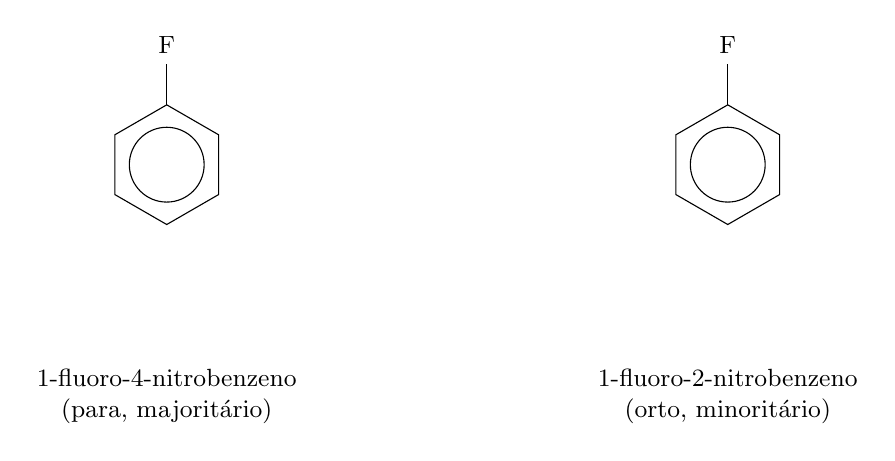
\begin{tikzpicture}[scale=0.95]
\def\r{0.8}
% para
\begin{scope}
\draw (90:\r)--(30:\r)--(-30:\r)--(-90:\r)--(-150:\r)--(150:\r)--cycle;
\draw (0,0) circle (0.5);
\draw (90:\r)--(90:1.35) node[above,font=\small]{F};
\begin{scope}[shift={(-90:\r)},rotate=-90]\nitro\end{scope}
\node[font=\small,align=center] at (0,-3.1) {1-fluoro-4-nitrobenzeno\\(para, majoritário)};
\end{scope}
% orto
\begin{scope}[xshift=7.5cm]
\draw (90:\r)--(30:\r)--(-30:\r)--(-90:\r)--(-150:\r)--(150:\r)--cycle;
\draw (0,0) circle (0.5);
\draw (90:\r)--(90:1.35) node[above,font=\small]{F};
\begin{scope}[shift={(30:\r)},rotate=30]\nitro\end{scope}
\node[font=\small,align=center] at (0,-3.1) {1-fluoro-2-nitrobenzeno\\(orto, minoritário)};
\end{scope}
\end{tikzpicture}
\end{center}
O outro produto é a água, $\mathrm{H_2O}$ (H--O--H, angular).

\medskip
\textbf{d)} As moléculas são (i) $\mathrm{H_2O}$; (ii) $\mathrm{H_2S}$; (iii) $\mathrm{CH_4O}$, que só pode ser o metanol $\mathrm{CH_3OH}$ (C com 4 ligações, O com 2, H com 1: estrutura única). Todas são polares, de massas molares pequenas e próximas; o que decide é a ligação de hidrogênio (H ligado a F, O ou N):
\begin{itemize}
\item $\mathrm{H_2S}$: o S é grande e pouco eletronegativo; a ligação S--H é pouco polar e a ligação de hidrogênio é desprezível. Só há dipolo--dipolo fraco e dispersão: menor ponto de ebulição ($\approx-60\,^\circ\mathrm{C}$; $\Delta H_{vap}\approx18{,}7\ \mathrm{kJ\,mol^{-1}}$).
\item $\mathrm{CH_3OH}$: um grupo O--H (1 H doador, 2 pares isolados no O) leva a $\approx2$ ligações de hidrogênio por molécula (cadeias e anéis); o grupo $\mathrm{CH_3}$, apolar, só acrescenta dispersão e atrapalha a formação de rede ($\approx65\,^\circ\mathrm{C}$; $\Delta H_{vap}\approx35\ \mathrm{kJ\,mol^{-1}}$).
\item $\mathrm{H_2O}$: 2 H doadores e 2 pares isolados receptores formam até 4 ligações de hidrogênio por molécula, em rede tridimensional. Maior ponto de ebulição ($100\,^\circ\mathrm{C}$; $\Delta H_{vap}\approx40{,}7\ \mathrm{kJ\,mol^{-1}}$), apesar da menor massa molar ($18$ contra $32$ e $34\ \mathrm{g\,mol^{-1}}$).
\end{itemize}
Assim, a massa molar não decide: o número e a eficiência das ligações de hidrogênio dominam.
\[
\mathrm{H_2S} < \mathrm{CH_3OH} < \mathrm{H_2O}\quad\Longleftrightarrow\quad \text{(ii)} < \text{(iii)} < \text{(i)}.
\]

\medskip
\noindent ANSWER: a) 3 arranjos ($\mathrm{SCN^-}$, $\mathrm{CNS^-}$, $\mathrm{CSN^-}$); b) $\mathrm{BF_3}$ (trigonal planar) e $\mathrm{NH_3}$ (pirâmide trigonal); c) nitração do fluorobenzeno: 1-fluoro-4-nitrobenzeno (majoritário) e 1-fluoro-2-nitrobenzeno (minoritário), mais $\mathrm{H_2O}$; d) (ii) $\mathrm{H_2S}$ $<$ (iii) $\mathrm{CH_3OH}$ $<$ (i) $\mathrm{H_2O}$.%
\newpage%
\section*{Questão 6}

\section*{Solução}

\textbf{Ferramenta.} Para um par ácido/base conjugado em água, a 25\,$^\circ$C, vale $K_a\cdot K_b=K_w=10^{-14}$, ou seja,
\[
pK_a+pK_b=14{,}00 .
\]
Cada espécie aparece em dois papéis (ácido e base), e cada papel tem o seu valor de $pK$.

\textbf{1) Valores de $pK_a$ e $pK_b$ das demais espécies.}

\begin{center}
\begin{tabular}{llcc}
Espécie (papel) & Par conjugado & $pK_a$ & $pK_b$ \\ \hline
$\mathrm{CH_3CCH}$ (ácido) & $\mathrm{CH_3CC^-}$ & $25{,}00$ (dado) & --- \\
$\mathrm{CH_3CC^-}$ (base) & $\mathrm{CH_3CCH}$ & --- & $14{,}00-25{,}00=-11{,}00$ \\
$\mathrm{H_2O}$ (base) & $\mathrm{H_3O^+}$ & --- & $15{,}70$ (dado) \\
$\mathrm{H_3O^+}$ (ácido) & $\mathrm{H_2O}$ & $14{,}00-15{,}70=-1{,}70$ & --- \\
$\mathrm{NH_3}$ (base) & $\mathrm{NH_4^+}$ & --- & $4{,}75$ (dado) \\
$\mathrm{NH_4^+}$ (ácido) & $\mathrm{NH_3}$ & $14{,}00-4{,}75=9{,}25$ & --- \\
$\mathrm{NH_2^-}$ (base) & $\mathrm{NH_3}$ & --- & $-22{,}00$ (dado) \\
$\mathrm{NH_3}$ (ácido) & $\mathrm{NH_2^-}$ & $14{,}00-(-22{,}00)=36{,}00$ & --- \\
\end{tabular}
\end{center}

\textbf{2) Constante de cada reação.} Todas as reações têm a forma $\mathrm{HA+B\rightleftharpoons A^-+BH^+}$. Ela é a diferença entre as reações $\mathrm{HA\rightleftharpoons H^++A^-}$ (constante $K_a(\mathrm{HA})$) e $\mathrm{BH^+\rightleftharpoons H^++B}$ (constante $K_a(\mathrm{BH^+})$). Logo
\[
K=\frac{K_a(\mathrm{HA})}{K_a(\mathrm{BH^+})}
\quad\Longrightarrow\quad
\log K=pK_a(\mathrm{BH^+})-pK_a(\mathrm{HA}) .
\]
Equivalentemente, $\log K=14{,}00-pK_a(\mathrm{HA})-pK_b(\mathrm{B})$. Se $K>1$ os produtos são favorecidos. Se $K<1$ os reagentes são favorecidos. O equilíbrio desloca-se para o lado do ácido mais fraco, ou seja, do maior $pK_a$.

\textbf{a) Reação 1:} $\mathrm{CH_3CCH+H_2O\rightleftharpoons CH_3CC^-+H_3O^+}$.

Aqui $\mathrm{HA}=\mathrm{CH_3CCH}$ e $\mathrm{BH^+}=\mathrm{H_3O^+}$.
\[
\log K_1=pK_a(\mathrm{H_3O^+})-pK_a(\mathrm{propino})=-1{,}70-25{,}00=-26{,}70
\;\Rightarrow\; K_1=10^{-26,70}\approx 2\times10^{-27}.
\]
Como $K_1\ll1$, o equilíbrio \textbf{não favorece} a formação dos produtos. O ácido mais forte é $\mathrm{H_3O^+}$ ($pK_a=-1{,}70$), que está no lado dos produtos, e o equilíbrio fica deslocado para os reagentes.

\textbf{b) Reação 2:} $\mathrm{CH_3CCH+NH_3\rightleftharpoons CH_3CC^-+NH_4^+}$.

Aqui $\mathrm{BH^+}=\mathrm{NH_4^+}$.
\[
\log K_2=pK_a(\mathrm{NH_4^+})-pK_a(\mathrm{propino})=9{,}25-25{,}00=-15{,}75
\;\Rightarrow\; K_2=10^{-15,75}\approx 1{,}8\times10^{-16}.
\]
Como $K_2\ll1$, o equilíbrio \textbf{não favorece} os produtos. A amônia é uma base fraca demais para desprotonar o propino, pois $\mathrm{NH_4^+}$ ($pK_a=9{,}25$) é muito mais ácido que o propino ($pK_a=25{,}00$).

\textbf{c) Reação 3:} $\mathrm{CH_3CCH+NaNH_2\rightleftharpoons CH_3CCNa+NH_3}$.

Os íons $\mathrm{Na^+}$ aparecem dos dois lados e são espectadores. A reação efetiva é $\mathrm{CH_3CCH+NH_2^-\rightleftharpoons CH_3CC^-+NH_3}$, em que $\mathrm{BH^+}$ é substituído por $\mathrm{NH_3}$ atuando como ácido conjugado de $\mathrm{NH_2^-}$.
\[
\log K_3=pK_a(\mathrm{NH_3})-pK_a(\mathrm{propino})=36{,}00-25{,}00=+11{,}00
\;\Rightarrow\; K_3=10^{11}.
\]
Verificação por $pK_b$: $14{,}00-25{,}00-(-22{,}00)=+11{,}00$, o mesmo resultado. Como $K_3\gg1$, o equilíbrio \textbf{favorece} fortemente os produtos. O ânion $\mathrm{NH_2^-}$ ($pK_b=-22{,}00$) é uma base muito mais forte que $\mathrm{CH_3CC^-}$ ($pK_b=-11{,}00$), e o propino ($pK_a=25$) é um ácido bem mais forte que a $\mathrm{NH_3}$ ($pK_a=36$).

\textbf{Conferência e observações.} Os sinais são coerentes: quanto mais negativo o $pK_b$, mais forte a base ($\mathrm{NH_2^-}$ é mais forte que $\mathrm{CH_3CC^-}$, que por sua vez é mais forte que $\mathrm{H_2O}$ e $\mathrm{NH_3}$). A relação $pK_a+pK_b=14$ vale para a escala aquosa a 25\,$^\circ$C. Valores fora da faixa de 0 a 14 (como $-1{,}70$, $25$ e $36$) são extrapolações formais, usadas aqui só para comparar a força relativa de ácidos e bases. Na prática, $\mathrm{NaNH_2}$ não pode ser usado em água, onde reage com o solvente, e sim em solvente menos ácido, como $\mathrm{NH_3}$ líquida.

\textbf{Resumo:} $pK_b(\mathrm{CH_3CC^-})=-11{,}00$; $pK_a(\mathrm{H_3O^+})=-1{,}70$; $pK_a(\mathrm{NH_4^+})=9{,}25$; $pK_a(\mathrm{NH_3})=36{,}00$.

ANSWER: $pK_b(\mathrm{CH_3CC^-})=-11{,}00$; $pK_a(\mathrm{H_3O^+})=-1{,}70$; $pK_a(\mathrm{NH_4^+})=9{,}25$; $pK_a(\mathrm{NH_3})=36{,}00$. (a) $K_1=10^{-26,70}$, não favorece os produtos. (b) $K_2=10^{-15,75}$, não favorece os produtos. (c) $K_3=10^{11}$, favorece os produtos.%
\newpage%
\section*{Questão 7}

\section*{Solução}

\textbf{Dados e ideia central.} Energia de um fóton de $\lambda=450\ \text{nm}$:
\[
E_f=\frac{hc}{\lambda}=\frac{6{,}63\times10^{-34}\cdot 3{,}0\times10^{8}}{4{,}50\times10^{-7}}=4{,}42\times10^{-19}\ \text{J}\ (\approx 2{,}76\ \text{eV}),
\qquad
N_A E_f=6{,}02\times10^{23}\cdot 4{,}42\times10^{-19}=2{,}66\times10^{5}\ \text{J}\cdot\text{mol}^{-1}.
\]
Cada fóton gera 1 elétron e cada $\text{H}_2$ exige 2 elétrons (item a). Logo, \emph{1 mol de $\text{H}_2$ consome 2 mol de fótons}.

O $\Delta H^\circ=+572\ \text{kJ}\cdot\text{mol}^{-1}$ refere-se à equação \emph{como escrita}, isto é, a 2 mol de $\text{H}_2$. Por mol de $\text{H}_2$ são $+286\ \text{kJ}$. Esse é o mínimo termodinâmico para qualquer processo de decomposição da água, independente do semicondutor. Como o enunciado só fornece $\Delta H^\circ$, é ele que se usa como energia da reação.

\medskip
\textbf{a) Semirreações.} O enunciado não fixa o meio. Apresento as duas formas, que são equivalentes. Em meio ácido:
\begin{align*}
\text{Cátodo (redução):}\quad & 4\,\text{H}^{+}(aq)+4\,e^{-}\rightarrow 2\,\text{H}_2(g)\\
\text{Ânodo (oxidação):}\quad & 2\,\text{H}_2\text{O}(\ell)\rightarrow \text{O}_2(g)+4\,\text{H}^{+}(aq)+4\,e^{-}
\end{align*}
Em meio básico:
\begin{align*}
\text{Cátodo:}\quad & 4\,\text{H}_2\text{O}(\ell)+4\,e^{-}\rightarrow 2\,\text{H}_2(g)+4\,\text{OH}^{-}(aq)\\
\text{Ânodo:}\quad & 4\,\text{OH}^{-}(aq)\rightarrow \text{O}_2(g)+2\,\text{H}_2\text{O}(\ell)+4\,e^{-}
\end{align*}
Igualados os 4 elétrons nas duas semirreações, a soma cancela elétrons e íons e resulta $2\,\text{H}_2\text{O}\rightarrow 2\,\text{H}_2+\text{O}_2$. São 4 elétrons para 2 mol de $\text{H}_2$, ou seja, 2 elétrons por $\text{H}_2$.

\medskip
\textbf{b) Energia da luz por mol de $\text{H}_2$.} São necessários 2 mol de fótons de 450 nm:
\[
E=2\,N_A\frac{hc}{\lambda}=2\cdot 2{,}66\times10^{5}\ \text{J}\approx 5{,}32\times10^{5}\ \text{J}\cdot\text{mol}^{-1}\ \Rightarrow\ \boxed{\approx 532\ \text{kJ por mol de H}_2}
\]
Esse valor é maior que o mínimo termodinâmico de 286 kJ. Isso é coerente, pois o fóton de 450 nm (2,76 eV) tem mais energia que os cerca de 1,48 eV por elétron ($=\Delta H/2F$) exigidos pela reação. O excesso de cada fóton é dissipado (por exemplo, como calor).

\medskip
\textbf{c) Quantidade máxima de $\text{H}_2$.} A potência incidente é $P=10\cdot0{,}2=2\ \text{W}$ e a energia em $t=3600\ \text{s}$ é $E=2\cdot3600=7{,}2\times10^{3}\ \text{J}$. Com eficiência quântica de 100\%, o limite é a \emph{contagem de fótons}:
\[
N=\frac{7{,}2\times10^{3}}{4{,}42\times10^{-19}}=1{,}63\times10^{22},
\qquad
n_{\text{fótons}}=\frac{1{,}63\times10^{22}}{6{,}02\times10^{23}}=2{,}71\times10^{-2}\ \text{mol}=n_{e^-}.
\]
Como $n_{\text{H}_2}=n_{e^-}/2$:
\[
n_{\text{H}_2}=\frac{2{,}71\times10^{-2}}{2}\approx \boxed{1{,}35\times10^{-2}\ \text{mol}}
\]
Conferência: $7{,}2\times10^{3}\ \text{J}\,/\,5{,}32\times10^{5}\ \text{J}\cdot\text{mol}^{-1}=1{,}35\times10^{-2}\ \text{mol}$.

O valor $7200/286000=2{,}5\times10^{-2}\ \text{mol}$ \emph{seria errado}. Ele supõe que toda a energia dos fótons vira energia de reação, ignorando que o excedente de cada fóton de 450 nm não gera mais $\text{H}_2$. De fato, $2{,}5\times10^{-2}$ mol de $\text{H}_2$ exigiria $5{,}0\times10^{-2}$ mol de elétrons, mais que os $2{,}71\times10^{-2}$ mol de fótons (elétrons) disponíveis.

\medskip
\textbf{d) Energia para 5,65 kg de $\text{H}_2$.} Com $M_{\text{H}_2}=2{,}02\ \text{g}\cdot\text{mol}^{-1}$:
\[
n_{\text{H}_2}=\frac{5650}{2{,}02}=2{,}797\times10^{3}\ \text{mol}.
\]
A pressão de 700 bar só afeta o armazenamento (trabalho de compressão, que o enunciado manda desprezar). Ela não altera a estequiometria nem a energia de produção, e por isso não distingue uma leitura da outra.

\emph{Leitura adotada.} O enunciado pede a energia mínima necessária ``pela fotodecomposição da água, \emph{utilizando o semicondutor}'', isto é, com o semicondutor de 450 nm descrito, em que cada fóton gera um elétron e cada $\text{H}_2$ exige 2 elétrons. Aqui ``mínima'' significa eficiência quântica de 100\% (nenhum fóton desperdiçado); qualquer célula real exigiria mais. A energia de luz é, então, a do item b):
\[
E=n_{\text{H}_2}\cdot 532\ \text{kJ}\cdot\text{mol}^{-1}=2{,}797\times10^{3}\cdot 5{,}32\times10^{2}\ \Rightarrow\ \boxed{E\approx 1{,}49\times10^{6}\ \text{kJ}}
\]
Essa leitura também dá sentido ao item e). Lá o enunciado introduz uma situação \emph{hipotética}, ``sem perdas'', em que a luz iguala a energia de combustão. Isso só é um caso diferente se em d) a luz de 450 nm fornecer mais energia que a combustão, como ocorre aqui.

\emph{Referência termodinâmica.} A energia armazenada no $\text{H}_2$ (e liberada na sua combustão) é
\[
E_{\Delta H}=n_{\text{H}_2}\cdot 286\ \text{kJ}\cdot\text{mol}^{-1}=2{,}797\times10^{3}\cdot286\approx 8{,}00\times10^{5}\ \text{kJ}.
\]
Esse é o limite inferior absoluto para qualquer processo, \emph{independente do semicondutor}. Ele só seria atingido se todo o excesso de energia de cada fóton fosse aproveitado, isto é, se não houvesse termalização. Com fótons de 450 nm a energia gasta é $1{,}49\times10^{6}\ \text{kJ}$, cerca de $1{,}9$ vez maior. Quem entender ``mínima'' como esse limite termodinâmico obtém $8{,}00\times10^{5}\ \text{kJ}$. Esse é o valor usado no item e).

\medskip
\textbf{e) Comprimento de onda máximo hipotético.} Invertendo a reação dada, a combustão $\text{H}_2+\tfrac12\text{O}_2\rightarrow\text{H}_2\text{O}(\ell)$ libera $286\ \text{kJ}\cdot\text{mol}^{-1}$. Usa-se $\text{H}_2\text{O}(\ell)$ porque é o estado do dado de $\Delta H^\circ$. Para $\text{H}_2\text{O}(g)$ seriam cerca de 242 kJ, valor que não é dado. Para a massa dada:
\[
E_{\text{comb}}=2{,}797\times10^{3}\cdot 286\ \text{kJ}\approx 8{,}00\times10^{5}\ \text{kJ}=8{,}00\times10^{8}\ \text{J}.
\]
Elétrons e fótons necessários (1:1, 2 elétrons por $\text{H}_2$):
\[
n_{\text{fótons}}=2\cdot 2{,}797\times10^{3}=5{,}594\times10^{3}\ \text{mol},
\qquad
N=5{,}594\times10^{3}\cdot 6{,}02\times10^{23}=3{,}37\times10^{27}\ \text{fótons}.
\]
Sem perdas, a energia total dos fótons é igual a $E_{\text{comb}}$. Logo, a energia de cada fóton é
\[
E_f=\frac{E_{\text{comb}}}{N}=\frac{8{,}00\times10^{8}}{3{,}37\times10^{27}}\approx 2{,}375\times10^{-19}\ \text{J}\ (\approx1{,}48\ \text{eV}),
\]
\[
\lambda_{\max}=\frac{hc}{E_f}=\frac{6{,}63\times10^{-34}\cdot3{,}0\times10^{8}}{2{,}375\times10^{-19}}\approx 8{,}37\times10^{-7}\ \text{m}=\boxed{\approx 837\ \text{nm}}
\]
\emph{Forma fechada.} Como $n_{\text{H}_2}$ se cancela, $\lambda_{\max}$ não depende da massa:
\[
\lambda_{\max}=\frac{2\,N_A\,h\,c}{|\Delta H|_{\text{por mol de }\text{H}_2}}=\frac{2\cdot 6{,}02\times10^{23}\cdot 6{,}63\times10^{-34}\cdot 3{,}0\times10^{8}}{2{,}86\times10^{5}}\approx 8{,}37\times10^{-7}\ \text{m}.
\]
Como $E_f=hc/\lambda$ diminui com $\lambda$, o semicondutor fornece energia suficiente apenas para $\lambda\le\lambda_{\max}$. Assim, 837 nm é o valor \emph{máximo}. Conferência: $\lambda_{\max}=450\cdot\dfrac{532{,}2}{286}\approx 837\ \text{nm}$, pois $\lambda\propto 1/E_f$. O valor, no infravermelho próximo, é maior que 450 nm, como esperado, já que agora não há excesso de energia por fóton.

\medskip
\textbf{Resumo:} (b) $\approx 532\ \text{kJ}\cdot\text{mol}^{-1}$ de $\text{H}_2$; (c) $\approx 1{,}35\times10^{-2}$ mol; (d) $\approx 1{,}49\times10^{6}\ \text{kJ}$ com fótons de 450 nm e eficiência quântica de 100\% (limite termodinâmico, independente do semicondutor: $8{,}00\times10^{5}\ \text{kJ}$); (e) $\approx 837\ \text{nm}$.

ANSWER: (a) Meio ácido: cátodo $4\text{H}^++4e^-\rightarrow2\text{H}_2$; ânodo $2\text{H}_2\text{O}\rightarrow\text{O}_2+4\text{H}^++4e^-$ (meio básico: cátodo $4\text{H}_2\text{O}+4e^-\rightarrow2\text{H}_2+4\text{OH}^-$; ânodo $4\text{OH}^-\rightarrow\text{O}_2+2\text{H}_2\text{O}+4e^-$). (b) $\approx 532\ \text{kJ}\cdot\text{mol}^{-1}$ de $\text{H}_2$. (c) $\approx 1{,}35\times10^{-2}$ mol de $\text{H}_2$. (d) $\approx 1{,}49\times10^{6}\ \text{kJ}$ com o semicondutor de 450 nm (limite termodinâmico, independente do semicondutor: $8{,}00\times10^{5}\ \text{kJ}$). (e) $\lambda_{\max}\approx 837\ \text{nm}$.%
\newpage%
\section*{Questão 8}

\section*{Solução}

\textbf{Hipóteses.} Os dados termodinâmicos não dependem de $T$ nem de $P$. A combustão é completa e só gera produtos gasosos, então a água sai como $\mathrm{H_2O(g)}$. Massas molares: $M(\mathrm{CH_4}) = 12{,}01 + 4\cdot 1{,}01 = 16{,}05\ \mathrm{g\cdot mol^{-1}}$ e $M(\mathrm{O_2}) = 32{,}00\ \mathrm{g\cdot mol^{-1}}$.

\textbf{a) Equação e entalpia de combustão}

\[
\mathrm{CH_4(g) + 2\,O_2(g) \longrightarrow CO_2(g) + 2\,H_2O(g)}
\]

Como o enunciado exige produtos gasosos, a entalpia de formação da água gasosa é
\[
\Delta H_f^{\circ}(\mathrm{H_2O,g}) = \Delta H_f^{\circ}(\mathrm{H_2O,\ell}) + \Delta H_{vap} = -286 + 45 = -241\ \mathrm{kJ\cdot mol^{-1}}.
\]

Pela lei de Hess, $\Delta H_c = \sum \Delta H_f(\text{produtos}) - \sum \Delta H_f(\text{reagentes})$:
\[
\Delta H_c = \left[-393 + 2(-241)\right] - \left[-75 + 2(0)\right] = -875 + 75 = -800\ \mathrm{kJ\cdot mol^{-1}}.
\]

A reação é exotérmica, e cada mol de $\mathrm{CH_4}$ libera $800\ \mathrm{kJ}$.

\textbf{b) Massas de combustível e oxidante}

O calor gerado na câmara é $12\ \mathrm{MJ} = 12000\ \mathrm{kJ}$. Então
\[
n_{\mathrm{CH_4}} = \frac{12000}{800} = 15\ \mathrm{mol}, \qquad n_{\mathrm{O_2}} = 2\cdot 15 = 30\ \mathrm{mol}.
\]
\[
m_{\mathrm{CH_4}} = 15\cdot 16{,}05 = 240{,}75\ \mathrm{g}, \qquad m_{\mathrm{O_2}} = 30\cdot 32{,}00 = 960\ \mathrm{g}.
\]

\textbf{c) Metano injetado na pré-câmara}

A turbobomba pressuriza o metano que será queimado na câmara principal, isto é, $240{,}75\ \mathrm{g}$. Ela deve gerar
\[
E_{\text{útil}} = 40\ \mathrm{J\cdot g^{-1}} \cdot 240{,}75\ \mathrm{g} = 9630\ \mathrm{J}.
\]

Com eficiência de $30\%$, o calor necessário na pré-câmara é
\[
Q_{\text{pré}} = \frac{9630}{0{,}30} = 32100\ \mathrm{J} = 32{,}1\ \mathrm{kJ}.
\]

Na pré-câmara há excesso de $\mathrm{O_2}$ (mistura rica em oxigênio), logo a combustão do metano é completa e libera os mesmos $800\ \mathrm{kJ\cdot mol^{-1}}$:
\[
n = \frac{32{,}1}{800} = 0{,}040125\ \mathrm{mol}
\quad\Rightarrow\quad
m_{\mathrm{CH_4(g)}} = 0{,}040125\cdot 16{,}05 \approx 0{,}644\ \mathrm{g}.
\]

Esse valor é cerca de $0{,}27\%$ do combustível total, coerente com a ``pequena porcentagem'' do enunciado.

\textbf{d) Massa mínima de $\mathrm{CH_4(\ell)}$ para refrigerar a tubeira}

A tubeira absorve
\[
Q = 0{,}25\% \cdot 12\ \mathrm{MJ} = 0{,}0025\cdot 12\cdot 10^{6}\ \mathrm{J} = 3{,}0\cdot 10^{4}\ \mathrm{J}.
\]

A massa é mínima quando o metano sofre o maior aquecimento possível, de $98\ \mathrm{K}$ até $188\ \mathrm{K}$, ou seja, $\Delta T = 90\ \mathrm{K}$. A transição de fase é desprezada, conforme o enunciado. Então
\[
Q = m\,c\,\Delta T
\quad\Rightarrow\quad
m_{\min} = \frac{3{,}0\cdot 10^{4}}{\dfrac{5}{3}\cdot 90} = \frac{3{,}0\cdot 10^{4}}{150} = 200\ \mathrm{g}.
\]

\textbf{Verificação.} Os $200\ \mathrm{g}$ são menores que os $240{,}75\ \mathrm{g}$ de metano da câmara principal. Isso é consistente, pois todo o metano de refrigeração é depois injetado na câmara. As unidades conferem: $\mathrm{J}/(\mathrm{J\cdot g^{-1}\cdot K^{-1}\cdot K}) = \mathrm{g}$. As ordens de grandeza também são plausíveis: $\sim 10^{2}\ \mathrm{g}$ de combustível por $12\ \mathrm{MJ}$ e frações de grama para a pré-câmara.

\textbf{Resultados:}
\begin{itemize}
\item[a)] $\mathrm{CH_4(g) + 2\,O_2(g) \rightarrow CO_2(g) + 2\,H_2O(g)}$, com $\Delta H_c = -800\ \mathrm{kJ\cdot mol^{-1}}$.
\item[b)] $m_{\mathrm{CH_4}} = 240{,}75\ \mathrm{g}$ e $m_{\mathrm{O_2}} = 960\ \mathrm{g}$.
\item[c)] $m \approx 0{,}644\ \mathrm{g}$ de $\mathrm{CH_4(g)}$.
\item[d)] $m_{\min} = 200\ \mathrm{g}$ de $\mathrm{CH_4(\ell)}$.
\end{itemize}

ANSWER: a) $\mathrm{CH_4 + 2\,O_2 \rightarrow CO_2 + 2\,H_2O(g)}$, $\Delta H_c = -800\ \mathrm{kJ\cdot mol^{-1}}$; b) $240{,}75\ \mathrm{g}$ de $\mathrm{CH_4}$ e $960\ \mathrm{g}$ de $\mathrm{O_2}$; c) $\approx 0{,}644\ \mathrm{g}$; d) $200\ \mathrm{g}$.%
\newpage%
\section*{Questão 9}

\section*{Solução}

\textbf{Leitura da figura.} Em (B), a camada azul está sob $\mathrm{Pt_1}$ (braço esquerdo) e a laranja sob $\mathrm{Pt_2}$ (braço direito). Entre cada placa e a cor há uma camada incolor de $\mathrm{H_2SO_4}$, portanto os dois eletrodos estão imersos na solução de ácido sulfúrico.

\medskip
\textbf{a) Espécies iônicas presentes.}

\begin{itemize}
\item $\mathrm{CuSO_4}$ dissocia-se em $\mathrm{Cu^{2+}}$ (na verdade $[\mathrm{Cu(H_2O)_6}]^{2+}$, azul) e $\mathrm{SO_4^{2-}}$.
\item $\mathrm{K_2Cr_2O_7}$ dissocia-se em $\mathrm{K^+}$ e $\mathrm{Cr_2O_7^{2-}}$ (laranja).
\item $\mathrm{H_2SO_4}$ ioniza-se em $\mathrm{H^+}$ (ou $\mathrm{H_3O^+}$) e $\mathrm{HSO_4^-}$. Este se ioniza em parte: $\mathrm{HSO_4^-} \rightleftharpoons \mathrm{H^+}+\mathrm{SO_4^{2-}}$.
\item A autoionização da água fornece traços de $\mathrm{OH^-}$.
\end{itemize}

Em meio ácido o equilíbrio $\mathrm{Cr_2O_7^{2-}+H_2O\rightleftharpoons 2\,CrO_4^{2-}+2\,H^+}$ está deslocado para a esquerda. Por isso a cor é laranja, e $\mathrm{CrO_4^{2-}}$ e $\mathrm{HCrO_4^-}$ existem só como traços.

\textbf{Espécies:} $\mathrm{Cu^{2+}},\ \mathrm{K^+},\ \mathrm{H^+},\ \mathrm{Cr_2O_7^{2-}},\ \mathrm{SO_4^{2-}},\ \mathrm{HSO_4^-},\ \mathrm{OH^-}$ (traços).

\medskip
\textbf{b) Origem das camadas colorida.}

Na região marrom coexistem $\mathrm{Cu^{2+}}$ (azul) e $\mathrm{Cr_2O_7^{2-}}$ (laranja), e a soma das cores dá marrom. $\mathrm{K^+}$, $\mathrm{SO_4^{2-}}$ e $\mathrm{H^+}$ são incolores. Esses íons não reagem entre si (ambos são oxidantes).

Sob o campo elétrico, os cátions migram para o catodo ($-$) e os ânions para o anodo ($+$):

\begin{itemize}
\item $\mathrm{Cu^{2+}}$ migra para o eletrodo do braço esquerdo, e $\mathrm{Cr_2O_7^{2-}}$ se afasta dele.
\item No braço esquerdo sobra apenas $\mathrm{Cu^{2+}}$ colorido, o que dá a camada \textbf{azul}.
\item No braço direito $\mathrm{Cr_2O_7^{2-}}$ migra para cima e $\mathrm{Cu^{2+}}$ desce. Sobra só dicromato, o que dá a camada \textbf{alaranjada}.
\item No fundo do U os dois íons ainda não se separaram, e a cor continua \textbf{marrom}.
\end{itemize}

As fronteiras ficam nítidas porque o $\mathrm{H_2SO_4}$ é um eletrólito incolor de alta condutividade e porque as soluções têm densidades diferentes. É a migração iônica (eletromigração) que separa as cores.

\medskip
\textbf{c) Anodo e catodo.}

O $\mathrm{Cu^{2+}}$ (cátion) foi para o braço de $\mathrm{Pt_1}$, logo $\mathrm{Pt_1}$ é o \textbf{catodo}. O $\mathrm{Cr_2O_7^{2-}}$ (ânion) foi para o braço de $\mathrm{Pt_2}$, logo $\mathrm{Pt_2}$ é o \textbf{anodo}.

Os eletrodos de $\mathrm{Pt}$ são inertes e estão mergulhados na camada de $\mathrm{H_2SO_4}$. Assim, as espécies que competem são as da solução ácida.

\emph{Catodo ($\mathrm{Pt_1}$), redução.} Em contato com o eletrodo só há $\mathrm{H^+}$ e $\mathrm{H_2O}$ para reduzir:
\[
2\,\mathrm{H^+(aq)}+2\,e^-\longrightarrow \mathrm{H_2(g)}\qquad (E^\circ=0{,}00\ \mathrm{V})
\]
O $\mathrm{Cu^{2+}}$ ($E^\circ=+0{,}34$ V) e o $\mathrm{Cr_2O_7^{2-}}$ ($E^\circ=+1{,}33$ V) seriam reduzidos antes do $\mathrm{H^+}$ se chegassem à placa. Porém o dicromato migra para o lado oposto, e na Figura (B) a frente azul ainda não alcançou $\mathrm{Pt_1}$ (há camada incolor entre elas). Se o $\mathrm{Cu^{2+}}$ alcançasse o catodo, passaria a depositar $\mathrm{Cu(s)}$ ($E^\circ=+0{,}34\ \mathrm{V}>0$).

\emph{Anodo ($\mathrm{Pt_2}$), oxidação.} O $\mathrm{SO_4^{2-}}$ só se oxidaria a $\mathrm{S_2O_8^{2-}}$ ($E^\circ\approx+2{,}01$ V). O $\mathrm{Cr(VI)}$ e o $\mathrm{Cu(II)}$ não se oxidam nessas condições. A oxidação da água é a mais fácil ($E^\circ_{\mathrm{red}}=+1{,}23$ V):
\[
2\,\mathrm{H_2O(\ell)}\longrightarrow \mathrm{O_2(g)}+4\,\mathrm{H^+(aq)}+4\,e^-
\]
Reação global (soma das semirreações, com o catodo multiplicado por 2): $2\,\mathrm{H_2O(\ell)}\to 2\,\mathrm{H_2(g)}+\mathrm{O_2(g)}$.

\medskip
\textbf{d) Polos da fonte e sentido da corrente.}

O catodo está ligado a $\mathrm{P_1}$. Este é o polo que fornece elétrons, portanto $\mathrm{P_1}$ é o polo \textbf{negativo}. O anodo está ligado a $\mathrm{P_2}$, que recebe os elétrons, portanto $\mathrm{P_2}$ é o polo \textbf{positivo}.

Sentido dos elétrons: $\mathrm{P_1}\to\mathrm{Pt_1}$ pelo fio, e $\mathrm{Pt_2}\to\mathrm{P_2}$ pelo fio.

A corrente elétrica convencional tem sentido contrário ao dos elétrons nos fios:
\[
\mathrm{P_2\,(+)}\to \mathrm{Pt_2}\to\text{solução}\to\mathrm{Pt_1}\to \mathrm{P_1\,(-)}
\]
Na solução a corrente vai de $\mathrm{Pt_2}$ para $\mathrm{Pt_1}$, ou seja, do anodo para o catodo.

\textbf{Verificação.} Os cátions ($\mathrm{Cu^{2+}}$, $\mathrm{H^+}$, $\mathrm{K^+}$) vão para $\mathrm{Pt_1}$ (catodo, $-$) e os ânions ($\mathrm{Cr_2O_7^{2-}}$, $\mathrm{SO_4^{2-}}$) vão para $\mathrm{Pt_2}$ (anodo, $+$). Isso é coerente com as cores observadas na Figura (B).

\medskip
ANSWER: a) $\mathrm{Cu^{2+}}$, $\mathrm{K^+}$, $\mathrm{H^+}$, $\mathrm{Cr_2O_7^{2-}}$, $\mathrm{SO_4^{2-}}$, $\mathrm{HSO_4^-}$, $\mathrm{OH^-}$ (traços); b) por migração iônica, $\mathrm{Cu^{2+}}$ vai ao catodo (azul) e $\mathrm{Cr_2O_7^{2-}}$ ao anodo (laranja); c) $\mathrm{Pt_1}$ é o catodo, com $2\,\mathrm{H^+}+2e^-\to \mathrm{H_2}$, e $\mathrm{Pt_2}$ é o anodo, com $2\,\mathrm{H_2O}\to \mathrm{O_2}+4\,\mathrm{H^+}+4e^-$; d) $\mathrm{P_1}$ é negativo e $\mathrm{P_2}$ é positivo, e a corrente convencional vai de $\mathrm{P_2}$ a $\mathrm{Pt_2}$, atravessa a solução até $\mathrm{Pt_1}$ e volta por $\mathrm{P_1}$.%
\newpage%
\section*{Questão 10}

\section*{Solução}

\textbf{Leis usadas.} Em qualquer decaimento nuclear conservam-se o número de massa (soma de prótons e nêutrons) e a carga (número atômico). Assim:
\begin{itemize}
\item emissão $\alpha$ ($^{4}_{2}\alpha$): o número de massa diminui de $4$ e o número atômico diminui de $2$;
\item emissão $\beta^-$ ($e^-$): o número de massa não muda e o número atômico aumenta de $1$, pois um nêutron vira próton;
\item isóbaros têm o mesmo número de massa, e isótonos têm o mesmo número de nêutrons, $N = A - Z$.
\end{itemize}

\textbf{Passo 1: identificar G (consideração iii).} O elemento $Q$ tem $A=232$ e $Z=89$. Após o decaimento $\beta^-$:
\[
{}^{232}_{89}Q \;\longrightarrow\; {}^{232}_{90}G + e^- + \bar{\nu}
\]
Logo $G$ tem $A=232$ e $Z=90$, e seu número de nêutrons é
\[
N_G = 232 - 90 = 142 .
\]

\textbf{Passo 2: identificar E (considerações ii e iv).} $E$ é isótono de $G$, então $N_E = N_G = 142$. Como $E$ tem $84$ prótons,
\[
A_E = Z_E + N_E = 84 + 142 = 226 .
\]

\textbf{Passo 3: identificar A (consideração i).} $A$ é isóbaro de $E$, então seu número de massa é $226$.

\subsection*{a) Valor de $X$}
\[
\boxed{X = 226}
\]

\subsection*{c) Número de partículas alfa}
O enunciado diz que $J$ ($A=238$) sofre apenas decaimentos $\alpha$. Cada emissão reduz a massa em $4$ u, e sendo $n$ o número de partículas $\alpha$:
\[
238 - 4n = 226 \;\Rightarrow\; n = \frac{238-226}{4} = 3 .
\]
\[
\boxed{n = 3}
\]
O resultado é inteiro, o que é coerente com a hipótese de só haver emissões $\alpha$.

\subsection*{b) Valor de $Z$}
Cada partícula $\alpha$ leva $2$ prótons, então
\[
Z = 92 - 2n = 92 - 2\cdot 3 = 86 .
\]
\[
\boxed{Z = 86}
\]

\textbf{Verificação.} A cadeia é
\[
{}^{238}_{92}J \xrightarrow{\;3\,\alpha\;} {}^{226}_{86}A .
\]
A massa se conserva: $238 = 226 + 3\cdot 4$. A carga também: $92 = 86 + 3\cdot 2$. $A$ ($Z=86$) é de fato isóbaro de $E$ ($Z=84$, $A=226$), pois ambos têm $A=226$. $E$ tem $226-84=142$ nêutrons, igual ao número de nêutrons de $G$, o que confirma a consistência dos dados. O número atômico $86$ corresponde ao radônio, isto é, $A = {}^{226}\mathrm{Rn}$.

ANSWER: a) $X = 226$; b) $Z = 86$; c) $3$ partículas alfa.%
\newpage%
\section*{Apêndice: parecer do avaliador}%
\subsection*{Questão 1: nota 9,2 (aprovada, rodada 1 de 1)}%
\textbf{Resposta da resolução às cegas do avaliador:} a) C(HA) na Solução 2 = 0,40 mol/L\newline%
b) C(HA) na Solução 1 = 2,0 mol/L\newline%
c) C(base) na Solução 3 = 0,80 mmol / 38 mL = 2/95 $\approx$ 2,1$\times$10$^{-}$$^2$ mol/L ($\approx$ 0,0211 mol/L)\newline%
\newline%
Chave do raciocínio: no ponto de equivalência só há o sal BA. A hidrólise de A$^{-}$ tem Kb = Kw/Ka = 10$^{-}$$^2$, {[}OH$^{-}${]} = {[}HA{]} = {[}A$^{-}${]} = 10$^{-}$$^2$ mol/L, então C\_sal = 2$\times$10$^{-}$$^2$ mol/L. Com V\_final = 40 mL, n = 0,80 mmol.\par %
As respostas finais coincidem com a referência: a) 0,40 mol/L; b) 2,0 mol/L; c) 2/95 $\approx$ 2,1$\times$10$^{-}$$^2$ mol/L. Refiz as contas e confirmei. Com pH = 12, {[}H?{]} = 10$^{-}$$^{1}$$^2$ e {[}OH$^{-}${]} = 10$^{-}$$^2$. Pelo balanço de carga exato, c\_s = 0,0200 mol/L. Daí C$_{2}$ = 20$\cdot$c\_s = 0,400 mol/L, C$_{1}$ = 2,00 mol/L e C$_{3}$ = 0,80 mmol/38 mL = 0,02105 mol/L. Conferi também que x$^2$/(c\_s - x) = 10$^{-}$$^2$ com c\_s = 0,02 dá x = 10$^{-}$$^2$ e pH = 12. O enunciado original foi relido e a leitura 'Solução I' = Solução 1 está certa. A resolução trata as armadilhas principais: não aproxima {[}A$^{-}${]} $\approx$ c\_s e adverte que isso daria o dobro do correto (hidrólise de 50\%), usa Kb = Kw/Ka = 10$^{-}$$^2$, usa V\_final = 40 mL, aplica o fator 5 na diluição no sentido certo e não inverte os volumes na estequiometria. Tem hipóteses explícitas (25 $^\circ$C, volumes aditivos, B? espectador), duas formas de fechar o balanço (massa e carga), unidades e algarismos significativos adequados. Os defeitos são de rigor e polimento: o balanço de prótons está implícito, a conferência da Solução 3 é pouco informativa e falta dizer que a concentração do ácido é a analítica. Nenhum afeta a correção. É uma resolução publicável como gabarito comentado, com pequenos ajustes.%
\begin{itemize}%
\item%
{[}minor{]} O balanço de prótons não é escrito. A resolução diz que {[}HA{]} = {[}OH$^{-}${]} pela estequiometria 1:1 da hidrólise e descarta a água, mas o correto é {[}OH$^{-}${]} = {[}HA{]} + {[}H?{]}. O termo {[}H?{]} = 10$^{-}$$^{1}$$^2$ é desprezível, e a justificativa só vale a ressalva. Deveria escrever a equação e comentar o termo desprezado, em vez de tratar {[}HA{]} = {[}OH$^{-}${]} como exata.%
\item%
{[}minor{]} A conferência da Solução 3 é fraca. Dizer que pH $\approx$ 12,3 é 'coerente com a mistura final em pH 12' não verifica nada de forma independente, porque a mistura tem pH 12 por hidrólise e a base pura teria pH 12,3. Uma checagem melhor seria recalcular o pH da mistura a partir de c\_s = 0,0200 e Kb = 10$^{-}$$^2$ (x$^2$/(c\_s - x) = 10$^{-}$$^2$ dá x = 10$^{-}$$^2$ e pH = 12). Isso fecha o ciclo sem ambiguidade.%
\item%
{[}minor{]} Não explicita que a concentração pedida do ácido é a analítica (total), e que a titulação consome também a fração ionizada. A resolução mostra {[}H?{]} $\approx$ 6$\times$10$^{-}$$^{7}$ mol/L na Solução 2, o que mostra que a ionização é desprezível, mas não tira a conclusão. É uma frase a acrescentar, não um erro.%
\item%
{[}minor{]} O balanço de carga é apresentado com '$\approx$' e {[}B?{]} = c\_s sem escrever o termo {[}H?{]}. Está correto, mas poderia ser dito que o fecho vale a menos de 10$^{-}$$^{1}$$^2$ mol/L. As hipóteses iniciais não listam as aproximações usadas (desprezar {[}H?{]} e a autoionização da água frente a 10$^{-}$$^2$), que aparecem só no meio do texto.%
\end{itemize}%
\subsection*{Questão 2: nota 9,2 (aprovada, rodada 1 de 1)}%
\textbf{Resposta da resolução às cegas do avaliador:} a) V(O2) = n$\cdot$R$\cdot$T/P = 0,025 mol $\times$ 0,0821 $\times$ 298 / 1 $\approx$ 0,61 L ($\approx$ 612 mL).\newline%
b) {[}H2O2{]}(5 min) = 0,5$\cdot$e\^{}(-0,0693$\cdot$5) = 0,5 $\times$ 0,707 $\approx$ 0,35 mol$\cdot$L$^{-}$$^{1}$ (0,3535).\par %
Conferi o enunciado na página 4 do PDF e refiz as contas em Python. (a) n(H2O2) = 0,05 mol, n(O2) = 0,025 mol e V = 0,025$\times$0,0821$\times$298 = 0,6116 L $\approx$ 0,61 L ($\approx$ 612 mL). (b) kt = 0,3465, {[}H2O2{]} = 0,5$\times$0,707 = 0,3535 $\approx$ 0,35 mol/L, com t$\frac12$ = 10 min e fator 1/$\surd$2 como checagem. As duas respostas coincidem com a minha referência e estão corretas. A convenção -d{[}H2O2{]}/dt = k{[}H2O2{]} é a pretendida: a tabela da prova fornece e\^{}(-0,3465) = 0,707, que só serve a esse caminho. A resolução trata bem as armadilhas: estequiometria 2:1, 22,4 L/mol (CNTP) rejeitado com checagem por Vm $\approx$ 24,5 L/mol, conversão $^\circ$C$\to$K, 1ª ordem justificada pela unidade de k, decaimento exponencial e não linear (checagem por meia{-}vida, 0,25 < 0,354 < 0,5), hipóteses de gás ideal, sem solubilidade de O2 e sem pressão de vapor, e conta numérica completa. Pontos fracos, todos menores: não cita a convenção alternativa que daria 0,25 mol/L, 'dado do enunciado' no lugar de 'dado da tabela de constantes', e pequena inconsistência de algarismos significativos (0,61 L e 612 mL). Não encontrei erro de conta nem de conceito. A resolução está próxima de um gabarito comentado publicável.%
\begin{itemize}%
\item%
{[}minor{]} A resolução fixa a convenção -d{[}H2O2{]}/dt = k{[}H2O2{]} como hipótese (iii) e a justifica pelo dado e\^{}(-0,3465)=0,707. Não menciona que, se k fosse definido pela velocidade da reação (v = -$\frac12$ d{[}H2O2{]}/dt), o resultado seria 0,25 mol/L. Um gabarito comentado deveria citar a alternativa e dizer por que foi descartada: a tabela de constantes fornece e\^{}(-0,3465) e a convenção usual por espécie dá 0,354. Mesmo assim a hipótese foi declarada explicitamente, o que cobre o ponto principal.%
\item%
{[}minor{]} Na 'Conferência' do item (b), a frase 'O dado e\^{}(-0,3465) do enunciado' é imprecisa. O dado está na tabela de constantes da prova, não no texto da questão (o corpo da solução diz corretamente 'dado da prova'). Usar essa constante para inferir a intenção do examinador é um argumento meta, não físico{-}químico. Convém apresentá{-}lo como indício, não como prova da convenção.%
\item%
{[}minor{]} Pequena inconsistência de algarismos significativos: 0,61 L (2 a.s.) aparece junto com '$\approx$ 612 mL' (3 a.s.) no resumo final, e 0,6116 L é arredondado para 0,61 L. Não afeta a correção (0,6116 L conferido). Seria mais limpo dar só 0,61 L $\approx$ 6,1$\times$10$^2$ mL e uma única precisão.%
\item%
{[}minor{]} O volume de O2 do item (a) não depende de k, nem da cinética além da conclusão de que a reação se completa. A resolução não diz isso explicitamente. Também não menciona que o catalisador não é consumido nem que o volume da solução é constante. A hipótese (i) cobre a parte essencial. Seriam acréscimos de rigor, não erros.%
\item%
{[}minor{]} A hipótese sobre T = 298 K (em vez de 298,15 K) é usada sem comentário. O resultado é o mesmo com 2 a.s. (0,6116 L contra 0,6120 L), então o efeito é nulo. A conta está correta e foi explicitada integralmente, como a prova exige.%
\end{itemize}%
\subsection*{Questão 3: nota 9,2 (aprovada, rodada 1 de 1)}%
\textbf{Resposta da resolução às cegas do avaliador:} a) t $\approx$ 553 s (V$_{1}$ = 1/$\surd$5 $\approx$ 0,447 L; evaporam $\approx$ 553 g de água; 540 cal/s ÷ 540 cal/g = 1 g/s). Com as constantes da prova, 552--554 s conforme o arredondamento.\newline%
b) Com V = V$_{1}$/2 $\approx$ 0,224 L: {[}B$^{-}${]} = ($\surd$15 - $\surd$5)$\cdot$10$^{-}$$^3$ $\approx$ 1,6$\cdot$10$^{-}$$^3$ mol/L e {[}A?{]} = ($\surd$15 + $\surd$5)$\cdot$10$^{-}$$^3$ $\approx$ 6,1$\cdot$10$^{-}$$^3$ mol/L (exatos: 1,637$\cdot$10$^{-}$$^3$ e 6,109$\cdot$10$^{-}$$^3$ M). O produto vale 10$^{-}$$^{5}$ = K\_PS, e a diferença {[}A?{]} - {[}B$^{-}${]} = 4,47$\cdot$10$^{-}$$^3$ M.\par %
As respostas finais do candidato coincidem com a referência e com minha verificação numérica. (a) V$_{1}$ = 1/$\surd$5 = 0,447 L, água evaporada $\approx$ 553 g, t = 540 cal/g $\cdot$ m ÷ 540 cal/s $\approx$ 553 s (exato 552,8 s). O candidato dá $\approx$554 s, usando $\surd$5 = 2,24 e 0,446 L, que é arredondamento aceitável. (b) V$_{2}$ = V$_{1}$/2 = 0,2236 L, saturação com balanço de massa: x = (3-$\surd$3)/2$\cdot$10$^{-}$$^3$ mol, {[}A?{]} = (1+$\surd$3)$\surd$5$\cdot$10$^{-}$$^3$ $\approx$ 6,1$\cdot$10$^{-}$$^3$ M e {[}B$^{-}${]} = ($\surd$3-1)$\surd$5$\cdot$10$^{-}$$^3$ $\approx$ 1,6$\cdot$10$^{-}$$^3$ M. Conferi com Python: x = 6,34$\cdot$10$^{-}$$^{4}$ mol, {[}A?{]} = 6,109$\cdot$10$^{-}$$^3$ M, {[}B$^{-}${]} = 1,637$\cdot$10$^{-}$$^3$ M, produto = 10$^{-}$$^{5}$ exatos. O enunciado original (página 5) foi relido e a leitura de \textbackslash{}"metade do volume do início da precipitação\textbackslash{}" = V$_{1}$/2 está correta. A resolução é bem estruturada: verifica Q$_{0}$ < K\_PS, usa P = $\Delta$H numericamente para conferência, descarta a raiz fisicamente impossível (y $\approx$ 2,37 > 1), usa as constantes $\surd$3 e $\surd$5 fornecidas e confere com a conservação de {[}A?{]}-{[}B$^{-}${]}. Os problemas são só de polimento: precisão do 554 vs 552,8 s, justificativa um pouco solta de atividade = concentração e K\_PS a 100 $^\circ$C, e falta de menção explícita às armadilhas (0,5 L; só concentrar os íons; {[}A?{]} = {[}B$^{-}${]} = $\surd$K\_PS). Nenhum erro de conta ou de conceito. Perto de um gabarito comentado, ligeiramente abaixo por esses detalhes de rigor e de discussão."%
\begin{itemize}%
\item%
{[}minor{]} Item (a): a resposta final é "$\approx$554 s" (553,6 s com $\surd$5 = 2,24 arredondado para 0,446 L), enquanto o valor exato é 1000$\cdot$(1-1/$\surd$5) = 552,8 s e a referência dá $\approx$553 s. A diferença (\textasciitilde{}1 s, 0,2\%) está dentro do arredondamento das constantes da prova, mas 0,446 L é 1/2,24 truncado, e o ideal seria indicar a faixa 553 $\pm$ 1 s ou o valor exato 552,8 s. O texto também mistura "$\approx$5,5$\cdot$10$^2$ s" com "$\approx$554 s", duas precisões diferentes para a mesma resposta.%
\item%
{[}minor{]} Justificativa de "atividade = concentração" é imprecisa: o enunciado diz que efeitos coligativos são desprezíveis, e isso (ponto de ebulição fixo em 100 $^\circ$C) não implica por si só atividade unitária do coeficiente de atividade. Faltou dizer explicitamente que o K\_PS é tomado como dado a 100 $^\circ$C, com AB(s) puro de atividade 1, e que o ponto de ebulição não sobe com a concentração, então não há calor sensível.%
\item%
{[}minor{]} A armadilha de interpretar "metade do volume correspondente ao do início da precipitação" como 0,5 L (metade do volume inicial) é evitada, mas a resolução não a menciona nem explica por que V$_{2}$ = V$_{1}$/2 $\approx$ 0,224 L e não 0,5 L. Também não diz que V$_{2}$ é atingido depois do início da precipitação (t $\approx$ 776 s), o que justificaria já haver sólido presente e a saturação. Uma frase resolveria.%
\item%
{[}minor{]} Item (b): não discute o erro clássico de só concentrar os íons (8,9$\cdot$10$^{-}$$^3$ e 4,5$\cdot$10$^{-}$$^3$ M, que dá Q = 4K\_PS). Embora a resolução use Q = 4K\_PS para justificar a precipitação, e a conferência com {[}A?{]}-{[}B$^{-}${]} = (nA-nB)/V$_{2}$ seja ótima, falta dizer explicitamente que o excesso de A? (10$^{-}$$^3$ mol) impede {[}A?{]} = {[}B$^{-}${]} = $\surd$K\_PS.%
\item%
{[}minor{]} Pequenas inconsistências de arredondamento: V$_{2}$ $\approx$ 0,223 L (1/4,48) contra 0,2236 L exato, e os resultados 6,1$\cdot$10$^{-}$$^3$ e 1,6$\cdot$10$^{-}$$^3$ M são dados com 2 algarismos, sem registrar os valores mais exatos (6,109$\cdot$10$^{-}$$^3$ e 1,637$\cdot$10$^{-}$$^3$ M). Isso não afeta a correção, mas um gabarito comentado traria o valor exato junto da aproximação.%
\end{itemize}%
\subsection*{Questão 4: nota 9,0 (aprovada, rodada 1 de 1)}%
\textbf{Resposta da resolução às cegas do avaliador:} a) m $\approx$ 5,58 g ($\approx$ 5,6 g) de NH$_{4}${[}NbO(C$_{2}$O$_{4}$)$_{2}${]}$\cdot$nH$_{2}$O. Em 10 g de BGN há 1,590 g de Nb$_{2}$O$_{5}$, que vêm de 1,590/0,285 de sal.\newline%
b) n = 9 (n calculado = 9,06; M\_sal $\approx$ 466,35 g/mol, o que dá NH$_{4}${[}NbO(C$_{2}$O$_{4}$)$_{2}${]}$\cdot$9H$_{2}$O).\par %
As respostas finais coincidem com as da minha referência. Item (a): $\approx$ 5,58 g (5,6 g). Item (b): n = 9. Refiz as contas em Python. Em 10 g de BGN há 1,590 g de Nb$_{2}$O$_{5}$, e a massa de sal é 1,590/0,285 = 5,58 g. M\_sal = 466,35 g/mol e M\_anidro = 303,00 g/mol, o que dá n = 9,065. Com n = 9, o resíduo seria 28,57\% e a massa de sal 5,56 g. O candidato trata bem as armadilhas principais. Converte \% molar de óxidos em massa usando as massas molares dos óxidos. Usa o fator 2 (2 sais para 1 Nb$_{2}$O$_{5}$). Entende que os 28,5\% se referem ao sal hidratado. Monta a fórmula C$_{4}$H$_{4}$NNbO$_{9}$ com 9 O. Mostra que o item (a) independe de n e traz a checagem cruzada com n = 9. A resolução é correta, completa e clara, com expressões numéricas resolvidas e as massas molares da tabela. Os defeitos são só de rigor e acabamento: falta comparar n = 8 e n = 10, falta checar o estado de oxidação +5 do Nb, a 'base de 100 mol de BGN' é mal formulada e a 'checagem de ordem de grandeza' é fraca. Nenhum deles afeta o resultado. Nota 9 porque a resolução serve de gabarito comentado, com pequenas melhorias possíveis.%
\begin{itemize}%
\item%
{[}minor{]} O item (b) mostra só que n=9 dá 28,57\%. Não mostra que n=8 (29,7\%) e n=10 (27,5\%) ficam fora da precisão de 28,5\%. Isso justificaria melhor o arredondamento de 9,07 para 9. O texto apenas afirma que n deve ser inteiro e que 28,57\% é compatível.%
\item%
{[}minor{]} A frase 'base de 100 mol de BGN' é imprecisa. Seria 100 mol de unidades{-}fórmula dos óxidos (60 SiO$_{2}$ + 36 CaO + 4 Nb$_{2}$O$_{5}$), porque o BGN é uma mistura/vidro de óxidos e não uma substância com fórmula única. Não afeta a conta.%
\item%
{[}minor{]} Não verifica que o Nb está no estado +5 no complexo (NH$_{4}$? +1, NbO$^3$? +3, 2 C$_{2}$O$_{4}$$^2$$^{-}$ -4). Esse é o argumento que liga o sal ao resíduo Nb$_{2}$O$_{5}$ e daria mais rigor à hipótese 'todo o Nb fica no resíduo'. A hipótese é afirmada na 'ideia geral', mas não é checada.%
\item%
{[}minor{]} O comentário de 'ordem de grandeza' (sal $\approx$ 28\% de Nb$_{2}$O$_{5}$, BGN $\approx$ 16\%) é vago e não valida nada de fato. Uma checagem melhor seria que o teor de Nb no sal é cerca de 19,9\% e que 5,6 g de sal para 10 g de BGN é plausível.%
\item%
{[}minor{]} O item (a) apresenta 5,58 g como resposta principal e 5,56 g (com n=9) como verificação. Isso deixa claro que o método usado foi o direto, com 28,5\%, mas o texto poderia dizer explicitamente que o item (a) independe do (b). A resposta final dá 5,58 g (5,6 g), o que é adequado.%
\end{itemize}%
\subsection*{Questão 5: nota 9,2 (aprovada, rodada 2 de 2)}%
\textbf{Resposta da resolução às cegas do avaliador:} Identificação: A = H, Z = B, X = C, G = N, R = O, Y = F, Q = S.\newline%
\newline%
a) **3 arranjos** (átomo central C, N ou S): {[}SCN{]}$^{-}$ (tiocianato/isotiocianato, o mais estável), {[}CNS{]}$^{-}$ e {[}CSN{]}$^{-}$. Cada sequência e sua reversa contam como um só arranjo.\newline%
\newline%
b) Trigonal planar: **BF$_{3}$** (também BH$_{3}$, SO$_{3}$, CH$_{2}$O). Pirâmide trigonal: **NH$_{3}$** (também NF$_{3}$).\newline%
\newline%
c) C$_{6}$H$_{5}$F (fluorbenzeno) sofre nitração eletrofílica, com F orientador orto/para. Produto principal: **p{-}fluornitrobenzeno** (1{-}fluoro{-}4{-}nitrobenzeno). Minoritário: o{-}fluornitrobenzeno. Subproduto: H$_{2}$O. Meta é desprezível e não ocorre dinitração a 25 $^\circ$C.\newline%
\newline%
d) **H$_{2}$S < CH$_{3}$OH < H$_{2}$O**, isto é, (ii) < (iii) < (i), com $\approx$ --60 $^\circ$C < $\approx$ 65 $^\circ$C < 100 $^\circ$C. A ordem vem da ligação de hidrogênio: nenhuma relevante no H$_{2}$S, 1 grupo O--H no metanol e rede de até 4 ligações por molécula na água.\par %
As respostas finais coincidem com a referência nos quatro itens: (a) 3 arranjos (SCN$^{-}$, CNS$^{-}$, CSN$^{-}$), (b) BF$_{3}$ e NH$_{3}$, (c) nitração do fluorobenzeno com 1{-}fluoro{-}4{-}nitrobenzeno majoritário, o{-}isômero minoritário e H$_{2}$O, (d) H$_{2}$S < CH$_{3}$OH < H$_{2}$O. Refiz as contas de cargas formais do item (a) e os valores batem: (0,0,--1)/(--1,0,0) para SCN$^{-}$, (--1,+1,--1) para CNS$^{-}$ e (--2,+2,--1) para CSN$^{-}$. Para a sequência C--S--N com octeto completo, mostrei que b1+b2 = 4 e que $\Sigma$|CF| = 5 em todas as estruturas. Compilei o TikZ do item (c) e os desenhos renderizam corretamente. O texto é completo e rigoroso: 16 e$^{-}$ de valência e isoeletrônico com CO$_{2}$, linear sp, ligante ambidentado (a diferença entre tiocianato e isotiocianato é só do lado de ligação, sem arranjo novo), anel triangular discutido e descartado, SEAr e não SNAr, explicação da orientação orto/para por ressonância C=F?, mononitração a 25 $^\circ$C, e ligação de hidrogênio como fator decisivo no item (d). Todas as armadilhas listadas foram tratadas: não contou 6 permutações, deu duas moléculas e não íons no item (b), não confundiu metanol com isômero, não pôs o metanol acima da água e indicou o para como majoritário. Só encontrei problemas menores: um argumento circular para o anel triangular, a equação simplificada do NO$_{2}$?, a frase 'massas próximas' e a ausência de menção ao octeto expandido do S. O resultado se aproxima de um gabarito comentado publicável. A incerteza residual é que a resposta '3' do item (a) depende de uma interpretação do enunciado que não consegui conferir com o gabarito oficial."%
\begin{itemize}%
\item%
{[}minor{]} Item (a): o descarte do anel triangular é parcialmente circular. O argumento 'contrário à geometria linear prevista para 16 elétrons' só vale para a conectividade em cadeia, e isso é justamente o que está em discussão. O argumento da tensão angular basta, e a contagem 'apenas cadeias abertas' deveria ser declarada como interpretação adotada. A resposta 3 é coerente com a referência, mas o enunciado ('arranjos atômicos') é ambíguo, e não consegui conferir com o gabarito oficial.%
\item%
{[}minor{]} Item (a): a afirmação 'nenhuma estrutura de octeto completo tem $\Sigma$|CF| < 5' está correta (verifiquei: o octeto completo exige b1+b2 = 4, e as três possibilidades dão $\Sigma$|CF| = 5). Ela ignora que o S, do 3º período, poderia expandir o octeto (por exemplo C$\equiv$S--N$^2$$^{-}$ com $\Sigma$|CF| = 3). A referência cita 'octeto incompleto/expandido'. Faltou dizer que mesmo com expansão a estrutura continua desfavorável, porque deixa N$^2$$^{-}$ ou carga muito alta. Também não aparece a forma S$\equiv$C--N$^2$$^{-}$ do SCN$^{-}$, que é dispensável.%
\item%
{[}minor{]} Item (c): o eletrófilo é gerado com a equação simplificada HNO$_{3}$ + H$_{2}$SO$_{4}$ ? NO$_{2}$? + HSO$_{4}$$^{-}$ + H$_{2}$O. Ela está balanceada e é aceitável. A versão completa, com 2 H$_{2}$SO$_{4}$ e formação de H$_{3}$O?, seria mais rigorosa, porque a água formada é protonada em meio de H$_{2}$SO$_{4}$ concentrado.%
\item%
{[}minor{]} Item (c): a explicação de para > orto usa o decaimento do efeito --I com a distância e diz que o impedimento estérico do F é pequeno. Isso é fisicamente mais correto do que a ênfase da referência na estérica, e o fator estatístico 2:1 é bem tratado. O candidato poderia ter explicitado que o para fica quase tão reativo quanto o benzeno (+M compensa --I) e que o orto é fortemente desativado. A faixa 10--15\% de orto está levemente alta para a literatura, mas dentro do tolerável.%
\item%
{[}minor{]} Item (c): o desenho compila e está correto (conferi o TikZ exato: para e orto com NO$_{2}$ em representação N?(=O)O$^{-}$, F no C1, legendas e rotulagem de majoritário/minoritário). No isômero orto o grupo nitro fica um pouco colado ao F. A água é só descrita em texto (H--O--H, angular), não desenhada. Isso não compromete a resposta.%
\item%
{[}minor{]} Item (d): a frase 'massas molares pequenas e próximas' é imprecisa, porque a água (18) difere de 32 e 34 g/mol. O próprio texto depois destaca a menor massa da água. Os dados (Teb $\approx$ --60 / 65 / 100 $^\circ$C; $\Delta$Hvap $\approx$ 18,7 / 35 / 40,7 kJ/mol) estão corretos e reforçam bem o argumento. Não menciona explicitamente que o metanol tem mais dispersão que a água, mas diz que a massa não decide.%
\end{itemize}%
\subsection*{Questão 6: nota 9,0 (aprovada, rodada 1 de 1)}%
\textbf{Resposta da resolução às cegas do avaliador:} Valores obtidos (com pKa + pKb = 14,00): pKb(CH$_{3}$CC$^{-}$) = -11,00; pKa(H$_{3}$O?) = -1,70; pKa(NH$_{4}$?) = 9,25; pKa(NH$_{3}$, como ácido) = 36,00.\newline%
\newline%
a) Reação 1: K = 10\^{}-26,70 $\approx$ 2$\times$10$^{-}$$^2$$^{7}$. NÃO favorece os produtos.\newline%
b) Reação 2: K = 10\^{}-15,75 $\approx$ 1,8$\times$10$^{-}$$^{1}$$^{6}$. NÃO favorece os produtos.\newline%
c) Reação 3: K = 10\^{}+11. FAVORECE fortemente os produtos (reação quase completa; só em meio não aquoso).\par %
Conferi o enunciado no PDF original (p. 8) e a transcrição está fiel. Refiz as contas e as respostas finais do candidato coincidem item por item com a minha referência. Valores: pKb(CH3CC$^{-}$) = -11,00; pKa(H3O?) = -1,70; pKa(NH4?) = 9,25; pKa(NH3) = 36,00. Constantes: K1 = 10\^{}-26,7 $\approx$ 2$\times$10$^{-}$$^2$$^{7}$ (não favorece); K2 = 10\^{}-15,75 $\approx$ 1,8$\times$10$^{-}$$^{1}$$^{6}$ (não favorece); K3 = 10$^{1}$$^{1}$ (favorece). Essas respostas estão corretas. O método é limpo e correto: K = Ka(HA)/Ka(BH?), log K = pKa(BH?) - pKa(HA). Há uma verificação cruzada por pKb em (c). Na Reação 3 o Na? é tratado como espectador, e o NH3 aparece com dois pKa distintos (9,25 como NH4? e 36,00 como ácido). Há comentário sobre a validade da escala aquosa e sobre NaNH2 só poder ser usado em NH3 líquida. A tabela de pK por espécie e papel responde claramente ao pedido de \textbackslash{}"determinar pKa e pKb das demais espécies\textbackslash{}". Os problemas encontrados são só de rigor e completude: falta justificar por que o pKb da água se refere ao par H2O/H3O?, a generalização HA + B ? A$^{-}$ + BH? não cobre literalmente a Reação 3, e a discussão do efeito nivelador poderia ser um pouco mais completa. Nenhuma das armadilhas listadas foi caída. Está próxima de um gabarito comentado publicável.%
\begin{itemize}%
\item%
{[}minor{]} O pKb{[}H2O{]} = 15,70 é rotulado na tabela como o da H2O atuando como base (par H2O/H3O?), mas a resolução não justifica essa leitura. Esta é a principal armadilha da questão: 14 - 15,70 poderia ser lido como pKa da água ácida ou pKb do OH$^{-}$. Bastaria uma frase dizendo que o dado se refere à protonação H2O $\to$ H3O?, e que pKa(H3O?) = -1,70 é coerente com o valor tabelado ($\approx$ -1,7), ou seja, -log 55,5 $\approx$ -1,74.%
\item%
{[}minor{]} Na seção 2, a resolução afirma que "todas as reações têm a forma HA + B ? A$^{-}$ + BH?". Isso não vale para a Reação 3, onde o ácido conjugado de NH2$^{-}$ é NH3, neutro. A resolução corrige isso na própria letra (c), mas a generalização inicial está imprecisa. Seria melhor escrever HA + B ? A$^{-}$ + HB, com HB = ácido conjugado de B.%
\item%
{[}minor{]} A relação pKa + pKb = 14 é aplicada a pares como CH3CCH/CH3CC$^{-}$ e NH3/NH2$^{-}$, que não existem em água por efeito nivelador. A resolução cita que são "extrapolações formais" e que NaNH2 reage com água, o que é bom. Mas não diz que, em água, o CH3CC$^{-}$ também seria protonado, nem que os valores de K das Reações 1 e 2 são formais por convenção (atividade da água = 1). Isso é um refinamento, não um erro.%
\item%
{[}minor{]} A justificativa de (c) é quantitativa (K = 10$^{1}$$^{1}$) e correta, mas poderia dizer explicitamente que a reação é praticamente completa, e que $\Delta$pKa = 11 unidades equivale a 11 ordens de grandeza. A conclusão de (a) e (b) está correta. Poderia reforçar que K $\approx$ 10$^{-}$$^2$$^{7}$ e 10$^{-}$$^{1}$$^{6}$ significam desprotonação desprezível, e que a Reação 2 é menos desfavorável que a 1, mas ainda muito desfavorável.%
\end{itemize}%
\subsection*{Questão 7: nota 9,0 (aprovada, rodada 3 de 3)}%
\textbf{Resposta da resolução às cegas do avaliador:} a) Cátodo (redução): 4 H? + 4 e$^{-}$ $\to$ 2 H$_{2}$ (em meio básico ou neutro: 4 H$_{2}$O + 4 e$^{-}$ $\to$ 2 H$_{2}$ + 4 OH$^{-}$). Ânodo (oxidação): 2 H$_{2}$O $\to$ O$_{2}$ + 4 H? + 4 e$^{-}$ (em meio básico: 4 OH$^{-}$ $\to$ O$_{2}$ + 2 H$_{2}$O + 4 e$^{-}$). Soma: 2 H$_{2}$O $\to$ 2 H$_{2}$ + O$_{2}$.\newline%
b) E\_fóton = 4,42$\times$10$^{-}$$^{1}$$^{9}$ J, ou 266 kJ por mol de fótons. Como 1 mol de H$_{2}$ exige 2 mol de e$^{-}$ (2 mol de fótons), a energia é $\approx$ 5,32$\times$10$^2$ kJ (5,32$\times$10$^{5}$ J) por mol de H$_{2}$.\newline%
c) Energia recebida = 2,0 W $\cdot$ 3600 s = 7,2$\times$10$^3$ J. Isso dá 1,63$\times$10$^2$$^2$ fótons, ou 2,71$\times$10$^{-}$$^2$ mol de e$^{-}$. Logo n(H$_{2}$) $\approx$ 1,35$\times$10$^{-}$$^2$ mol.\newline%
d) n(H$_{2}$) = 5650/2,02 $\approx$ 2,80$\times$10$^3$ mol. E\_mín = n $\cdot$ 286 kJ/mol $\approx$ 8,0$\times$10$^{5}$ kJ = 8,0$\times$10$^{8}$ J. (Leitura alternativa, com fótons de 450 nm: $\approx$ 1,5$\times$10$^{6}$ kJ.)\newline%
e) A energia da combustão é 8,0$\times$10$^{8}$ J, e são 5594 mol de fótons (3,37$\times$10$^2$$^{7}$). Logo E\_fóton = 2,375$\times$10$^{-}$$^{1}$$^{9}$ J e $\lambda$\_máx $\approx$ 8,4$\times$10$^2$ nm (837 nm).\par %
Os itens (a), (b), (c) e (e) coincidem com a minha referência e foram conferidos em Python: (b) 532 kJ por mol de H$_{2}$; (c) 1,35$\times$10$^{-}$$^2$ mol; (e) 837 nm. Em (a), as semirreações em meio ácido e em meio básico estão balanceadas (4 e$^{-}$) e somam 2 H$_{2}$O $\to$ 2 H$_{2}$ + O$_{2}$. Em (d), o candidato destaca 1,49$\times$10$^{6}$ kJ (532 kJ/mol $\times$ 2797 mol) e cita 8,00$\times$10$^{5}$ kJ como limite termodinâmico. A minha referência faz o contrário. Os dois valores aparecem nas duas resoluções, então a divergência é só de qual entra como resposta principal.\newline%
\newline%
Refiz o item (d) e considero a leitura do candidato defensível, talvez mais provável que a da referência. O enunciado diz "energia mínima necessária \ldots{} utilizando o semicondutor". Esse "utilizando o semicondutor" só faz sentido se a resposta depender do semicondutor, e o limite termodinâmico ($\Delta$H) não depende. O item (d) também é o inverso do item (c): em (c) calcula{-}se o H$_{2}$ máximo com eficiência quântica de 100\% e, em (d), a energia mínima de luz para uma dada massa de H$_{2}$, ou seja, 2 fótons de 450 nm por H$_{2}$. A leitura termodinâmica (8,0$\times$10$^{5}$ kJ) continua possível, porque "mínima" lembra $\Delta$H e o enunciado fornece $\Delta$H. Por isso não afirmo que a reposta do candidato é a única correta, mas ela é plausível e honestamente justificada.\newline%
\newline%
A resolução é completa, tem expressões numéricas explícitas, unidades coerentes e conferências cruzadas (7200 J / 532 kJ/mol; 450$\cdot$532,2/286). Também trata as armadilhas: $\Delta$H refere{-}se a 2 mol de H$_{2}$ (286 kJ/mol), 2 mol de e$^{-}$ por H$_{2}$, 7200/286000 violando o limite de fótons, M(H$_{2}$) = 2,02, H$_{2}$O(?) e não H$_{2}$O(g), os 700 bar como distração, e $\lambda$ como limite máximo. Os defeitos restantes são pequenos.%
\begin{itemize}%
\item%
{[}minor{]} Item (d): a resposta final traz dois valores (1,49$\times$10$^{6}$ kJ e 8,00$\times$10$^{5}$ kJ). A leitura adotada está bem justificada, mas uma banca prefere um único valor definitivo. Se o gabarito oficial for o limite termodinâmico, o valor principal do candidato pode perder pontos, e a menção ao outro só rende crédito parcial. Convém deixar o valor principal mais destacado e a alternativa apenas como observação.%
\item%
{[}minor{]} Item (d): o argumento de que a leitura 'também dá sentido ao item e)' e de que 'isso só é um caso diferente se em d) a luz de 450 nm fornecer mais energia' é frágil. Sob a leitura termodinâmica, (e) também é um caso distinto. Esse trecho deveria ser reduzido ou apresentado como indício, não como prova. O argumento mais forte, que o candidato não destaca, é o paralelo com (c): eficiência quântica de 100\% e fótons de 450 nm.%
\item%
{[}minor{]} Item (d): 'só seria atingido se todo o excesso de energia de cada fóton fosse aproveitado, isto é, se não houvesse termalização' é uma explicação qualitativa pouco precisa. O limite termodinâmico seria atingido com fótons de energia igual a $\Delta$H/2 por elétron (o que o item (e) calcula), não aproveitando o excesso de fótons de 450 nm.%
\item%
{[}minor{]} Exigência da prova de resolver integralmente as expressões numéricas: em (d) e (e) alguns passos usam valores intermediários arredondados (532 kJ/mol, 2,375$\times$10$^{-}$$^{1}$$^{9}$ J) em vez de uma única expressão completa com h, c, N\_A e $\lambda$. A forma fechada de (e) está certa. Os resultados não mudam: 1,488$\times$10$^{6}$ kJ com valores exatos contra 1,49$\times$10$^{6}$ kJ, e 837,3 nm.%
\item%
{[}minor{]} Item (a): o candidato apresenta meio ácido e meio básico, o que é correto, mas não escolhe um como principal nem comenta qual meio é típico da célula fotoeletroquímica. É mais cuidado que erro, e não afeta a correção.%
\end{itemize}%
\subsection*{Questão 8: nota 9,0 (aprovada, rodada 1 de 1)}%
\textbf{Resposta da resolução às cegas do avaliador:} a) CH4(g) + 2 O2(g) $\to$ CO2(g) + 2 H2O(g); $\Delta$H\_comb = -800 kJ/mol de CH4 (-890 kJ/mol seria com H2O(l); soma{-}se 2$\cdot$45 kJ para a água gasosa).\newline%
b) m(CH4) = 15 mol $\cdot$ 16,05 g/mol $\approx$ 240,75 g ($\approx$ 240 g); m(O2) = 30 mol $\cdot$ 32,00 g/mol = 960 g.\newline%
c) m(CH4) na pré{-}câmara $\approx$ 0,644 g ($\approx$ 0,64 g). Q\_pré = 40 $\cdot$ 240,75 / 0,30 = 32,1 kJ; 32,1 / 800 = 0,0401 mol.\newline%
d) m\_mín(CH4(l)) = 30 000 J / (150 J/g) = 200 g.\par %
Reli o enunciado no PDF (p. 10) e refiz as contas em python. A resolução do candidato está correta em todos os itens e coincide com a minha referência. (a) CH4 + 2 O2 $\to$ CO2 + 2 H2O(g), com $\Delta$H = -800 kJ/mol. O candidato lê corretamente que 'apenas produtos gasosos' implica água gasosa e usa $\Delta$Hf(H2O,g) = -241. (b) 15 mol de CH4 = 240,75 g e 30 mol de O2 = 960 g. (c) 40$\cdot$240,75 = 9630 J; dividido por 0,30 dá 32,1 kJ; dividido por 800 kJ/mol dá 0,040125 mol, ou 0,644 g. O candidato divide por 0,30 (não multiplica), converte o calor em massa de CH4 e bombeia só o combustível da câmara principal. Esse valor é o mesmo da referência. A leitura alternativa, circular, daria 0,646 g, diferença de 0,3\%. (d) 0,25\% de 12 MJ = 30 kJ; c$\cdot$$\Delta$T = (5/3)$\cdot$90 = 150 J/g; m\_mín = 200 g. A transição de fase é ignorada e a mínima corresponde ao aquecimento até 188 K. A apresentação é clara, com unidades conferidas, contas integralmente resolvidas e uma verificação de coerência (200 g < 240,75 g; 0,27\% de combustível na pré{-}câmara). Os pontos fracos são de rigor expositivo: a hipótese de que a bomba não atua sobre o CH4 da pré{-}câmara não é declarada como hipótese, a leitura alternativa não é mencionada, e a armadilha de -890 kJ/mol não é comentada. Nada disso altera nenhum resultado. Nota 9 por estar no nível de um gabarito comentado, faltando só essas explicitações."%
\begin{itemize}%
\item%
{[}minor{]} Item (c): a hipótese central, de que a bomba trabalha só sobre os 240,75 g que vão para a câmara principal, aparece como afirmação e não como hipótese explícita. O texto não diz que o CH4 da pré{-}câmara entra já vaporizado (CH4(g) na figura) e não é bombeado. Também não menciona a leitura alternativa, em que o metano da pré{-}câmara entra na massa bombeada e o resultado sai 0,646 g (cerca de 0,3\% de diferença). Um gabarito comentado deveria declarar a hipótese e dizer que a alternativa praticamente não muda o resultado.%
\item%
{[}minor{]} Item (c): o texto assume que o calor da pré{-}câmara vale 800 kJ/mol, com H2O(g), mas não diz que esse calor não entra nos 12 MJ da câmara principal. Também não diz que o CH4 da pré{-}câmara é adicional aos 15 mol do item (b), e não parte deles. O argumento do excesso de O2 só justifica a combustão completa. Falta mencionar que, com dados independentes de T e P, o $\Delta$H por mol de CH4 é o mesmo nas duas câmaras.%
\item%
{[}minor{]} Item (a): o enunciado dá H2O(l) e a água gasosa foi obtida corretamente (-286 + 45 = -241). O texto não faz a conferência com H2O(l) (-890 kJ/mol, que sairia da mesma conta sem a água vaporizada). Também não alerta que usar -890 é o erro previsível, e que ele se propagaria para (b) com 216 g de CH4 e para (c). Uma frase explicando por que a água sai como gás deixaria a justificativa mais didática.%
\item%
{[}minor{]} Item (b): a massa de CH4 depende da massa molar adotada (16,05 ou 16 g/mol). O texto declara 16,05 nas hipóteses, o que é correto, mas não registra que o valor arredondado ($\approx$240 g) também seria aceitável. Item (d): a razão de $\Delta$T = 90 K ser o aquecimento máximo está dita, mas a ideia de que a saída a temperatura menor exigiria mais massa poderia ser explicitada. O texto usa 'Q' para o calor da tubeira e, antes, para o calor da pré{-}câmara, o que é pouco prejudicial.%
\item%
{[}minor{]} A linha ANSWER final do item (a) omite os estados físicos de CH4, O2 e CO2 e só indica (g) na água. O corpo da solução tem a equação completa, então o dano é pequeno.%
\end{itemize}%
\subsection*{Questão 9: nota 9,0 (aprovada, rodada 1 de 1)}%
\textbf{Resposta da resolução às cegas do avaliador:} a) Cu2+, K+, Cr2O7\^{}2{-}, SO4\^{}2{-}, H+ (H3O+), além de HSO4{-} e OH{-} (e traços de HCrO4{-}/CrO4\^{}2{-}). b) Migração iônica: Cu2+ (azul) vai ao catodo e Cr2O7\^{}2{-} (alaranjado) ao anodo; no braço do catodo sobra só Cu2+ (faixa azul), no do anodo sobra só Cr2O7\^{}2{-} (faixa alaranjada); a base, com ambos, continua marrom. c) Pt1 = catodo: 2H+ + 2e{-} {-}> H2(g); Pt2 = anodo: 2H2O {-}> O2(g) + 4H+ + 4e{-} (global: 2H2O {-}> 2H2 + O2). d) P1 negativo, P2 positivo; corrente convencional: P2 {-}> Pt2 {-}> solução (direita para esquerda) {-}> Pt1 {-}> P1 (sentido horário na figura); elétrons no circuito externo em sentido contrário (P1 {-}> Pt1 e Pt2 {-}> P2).\par %
Reli a página 11 do enunciado e a Figura (B). A faixa azul está sob Pt1, no braço esquerdo, e a alaranjada sob Pt2, no braço direito, ambas separadas dos eletrodos por camada incolor de H2SO4. Os fios ligam P1--Pt1 e P2--Pt2 sem se cruzar. A leitura da figura pelo candidato está correta. Item a: Cu2+, K+, H+, Cr2O7\^{}2{-}, SO4\^{}2{-}, HSO4{-} e OH{-} (traços), com o equilíbrio cromato/dicromato bem tratado e sem listar espécies não iônicas; coincide com a referência. Item b: explica corretamente por migração iônica, com Cu2+ (azul) indo ao catodo e Cr2O7\^{}2{-} ao anodo, sobrando só um íon colorido em cada braço. A base marrom mantém os dois, e o candidato nota que K+, SO4\^{}2{-} e H+ são incolores. Item c: Pt1 é catodo (2H+ + 2e{-} $\to$ H2) e Pt2 é anodo (2H2O $\to$ O2 + 4H+ + 4e{-}), com a reação global balanceada. O candidato justifica pela posição dos eletrodos na camada de H2SO4, discute os potenciais (Cu2+ 0,34 V, Cr2O7\^{}2{-} 1,33 V, O2/H2O 1,23 V, S2O8\^{}2{-}/SO4\^{}2{-} 2,01 V) e ressalva o que ocorreria se o Cu2+ chegasse ao catodo. Item d: P1 negativo e P2 positivo, corrente convencional P2$\to$Pt2$\to$solução$\to$Pt1$\to$P1, e elétrons no sentido oposto nos fios. Tudo isso confere com a minha referência e com a leitura da figura; não encontrei erro de química, de balanceamento ou de sinal. As armadilhas da referência foram tratadas: catodo pelas cores e posição, H2 em vez de Cu/Cr3+, migração em vez de reação, 2H2O em meio ácido e não 4OH{-}, polo positivo ligado ao anodo, e corrente convencional diferente do fluxo de elétrons. Os defeitos são só de acabamento: resposta mais longa que o \textbackslash{}"sucinta\textbackslash{}" pedido, justificativa frágil para a nitidez das fronteiras, e o circuito da corrente não fechado dentro da fonte nem descrito como horário. Resolução de qualidade próxima à de um gabarito comentado.%
\begin{itemize}%
\item%
{[}minor{]} Item (b): o enunciado pede explicação "sucinta", e a resposta é mais longa que o necessário. A justificativa de que as fronteiras ficam nítidas "porque o H2SO4 é um eletrólito de alta condutividade e porque as soluções têm densidades diferentes" é só plausível e fica solta. A densidade explica a estratificação H2SO4/mistura, mas não a nitidez das fronteiras móveis entre as zonas coloridas. Isso não afeta a resposta pedida, e deveria ser enxugado ou omitido.%
\item%
{[}minor{]} Item (d): a direção da corrente está correta (convencional P2$\to$Pt2$\to$solução, de Pt2 para Pt1, $\to$Pt1$\to$P1), mas não fecha o circuito dentro da fonte (P1$\to$P2) nem diz o sentido na figura (horário). Também não diz explicitamente que, na solução, a corrente é iônica. O bloco "Verificação" cobre em parte esse último ponto, ao citar cátions$\to$Pt1 e ânions$\to$Pt2.%
\item%
{[}minor{]} Item (c): o argumento de que o Cu2+ e o dicromato não chegam à Pt1 (há camada incolor e o dicromato migra para longe) está correto e é o ponto{-}chave. Falta dizer que K+ nunca se reduz em meio aquoso e que o Cr(VI) já está no estado máximo de oxidação. A resposta menciona o Cr(VI) só de passagem, no anodo. Os potenciais padrão são citados de memória, sem tabela no enunciado, o que é aceitável.%
\item%
{[}minor{]} Item (a): HCrO4{-} e CrO4\^{}2{-} são citados como traços no texto, mas ficam fora da lista final em negrito. Isso é coerente com a referência (lista mínima ou ampliada), mas a lista final poderia ter incluído H3O+ $\equiv$ H+ e esses traços entre parênteses.%
\end{itemize}%
\subsection*{Questão 10: nota 9,5 (aprovada, rodada 1 de 1)}%
\textbf{Resposta da resolução às cegas do avaliador:} a) X = 226. b) Z = 86 (A = $^2$$^2$$^{6}$$_{8}$$_{6}$Rn). c) 3 partículas alfa.\par %
Conferi o enunciado no PDF (página 12): a transcrição está fiel. As respostas finais coincidem com a minha referência: X = 226, Z = 86 e 3 partículas $\alpha$. Refiz as contas e estão certas. G tem A = 232 e Z = 90, logo N\_G = 142. Como E é isótono de G, N\_E = 142 e A\_E = 84 + 142 = 226. Como A é isóbaro de E, X = 226. Então n = (238 - 226)/4 = 3 e Z = 92 - 2$\cdot$3 = 86 (Rn{-}226). O sentido do $\beta$$^{-}$ está correto (A fixo, Z + 1), assim como $\alpha$ (A - 4, Z - 2). A distinção entre isóbaro e isótono está correta. O candidato não confundiu Z de A (86) com Z de E (84). Ele fez a verificação cruzada de massa e carga e conferiu que E (226 - 84 = 142 nêutrons) é de fato isótono de G. O raciocínio é passo a passo, com as expressões numéricas resolvidas, como a instrução 8 exige. As falhas são só de forma: ordem dos itens (a, c, b), falta de ressalva sobre a hipótese só{-}$\alpha$ frente à série real do U{-}238 e ausência dos nuclídeos intermediários. Está perto de um gabarito comentado publicável.%
\begin{itemize}%
\item%
{[}minor{]} Os itens foram resolvidos na ordem a), c), b), e não na ordem do enunciado. A ordem é lógica, porque Z depende de n, mas o corretor precisa procurar o item b) depois do c). Seria mais claro apresentar a)--c) na ordem pedida ou avisar da inversão no início.%
\item%
{[}minor{]} Não comenta que a cadeia só com emissões $\alpha$ é uma hipótese da questão: na série natural real do U{-}238 também ocorrem emissões $\beta$. Também não comenta que o enunciado chama de 'elemento' o que é um nuclídeo. Uma ressalva de uma linha deixaria a resolução mais rigorosa, sem contestar o enunciado.%
\item%
{[}minor{]} A cadeia final é dada só como $^2$$^3$$^{8}$$_{9}$$_{2}$J $\to$(3$\alpha$) $^2$$^2$$^{6}$$_{8}$$_{6}$A. Os nuclídeos intermediários ($^2$$^3$$^{4}$Th, $^2$$^3$$^{0}$Ra) não aparecem. Isso não é necessário para a resposta, mas daria uma verificação passo a passo mais completa.%
\item%
{[}minor{]} A distinção entre isóbaro, isótono e isótopo está nas leis iniciais, e a diferença Z\_A = 86 $\neq$ Z\_E = 84 aparece na verificação. Mas o texto não adverte explicitamente que A e E são elementos diferentes (Rn e Po) e que a condição i) fixa só o número de massa. Essa armadilha é tratada de forma implícita, não explícita.%
\end{itemize}%
\end{document}